\documentclass[
a4paper,                        % paper size
11pt,                           % font size
twoside,                        % two sided
footsepline,                    % add a line to separate the footer
headsepline,                    % add a line to separate the header
headexclude,                    % header does not belong to the text
footexclude,                    % footer does not belong to the text
pagesize,                       % set the pagesize in a DVI document
bibtotocnumbered,               % add the bibliography to the TOC
idxtotoc                        % add the index to the TOC
%openright,                      % start a new chapter on the right page
%,DIV12
%,draft
]{scrreprt}

\usepackage{nameref}            % nameref, varioref, hyperref must be
                                % used in this order (see hyperref
                                % README)!
\usepackage[draft]{varioref}    % defines \vref
\usepackage[bookmarksopen=true]
{hyperref}                      % automatically creates links when
                                % using pdflatex, defines \url
\usepackage{ifpdf}              % defines \ifpdf
\usepackage{graphicx}           % handles graphics
\usepackage{makeidx}            % creates the index
\usepackage{color}              % use colors

\usepackage{verbatim}           % required for \verbatim and \endverbatim
\usepackage{alltt}              % almost verbatim environment (code)
\usepackage{tocloft}            % required for the quickref
\usepackage{calc}               % compute length
\usepackage{ifthen}             % provide ifthen

%%%%%%%%%%%%%%%%%%%%%%%%%%%%%%%%%%%%%%%%%%%%%%%%%%
%%%%%%%%%%%%%%%%%%%%%%%%%%%%%%%%%%%%%%%%%%%%%%%%%%
%%%%%%%%% New Commands and Environments %%%%%%%%%%
%%%%%%%%%%%%%%%%%%%%%%%%%%%%%%%%%%%%%%%%%%%%%%%%%%
%%%%%%%%%%%%%%%%%%%%%%%%%%%%%%%%%%%%%%%%%%%%%%%%%%
\newcommand{\es}{\mbox{\textsf{ESPResSo}}}
\newcommand{\ie}{\textit{i.e.\/}}
\newcommand{\eg}{\textit{e.g.\/}}
\newcommand{\etal}{\textit{et al.\/}}

\newcommand{\codebox}[1]%
{\fcolorbox[rgb]{0,0,0}{0.9,0.9,0.9}{\ttfamily#1}}

\newsavebox{\thecodebox}
\newenvironment{code}{
  \begin{lrbox}{\thecodebox}
    \begin{minipage}{\linewidth-2em}
      \begin{alltt}
      }{
      \end{alltt}
    \end{minipage}
  \end{lrbox}
  \smallskip
  \begin{addmargin}[1em]{0pt}
    \codebox{\usebox{\thecodebox}}
  \end{addmargin}
  \smallskip
}

\makeatletter
\newenvironment{tclcode}
{
  \addtolength{\linewidth}{-2em}% set the line length
  \@minipagetrue%%%DPC%%%
  \@tempswatrue%%%DPC%%%
  \hsize=\linewidth%
  \setbox0=\vbox\bgroup\verbatim
}{\endverbatim
  \unskip\setbox0=\lastbox%%%DPC%%%
  \egroup
  \par
  \smallskip
  \noindent
  \begin{addmargin}[1em]{0pt}
    \codebox{\box0}
  \end{addmargin}
  \par
  \smallskip
  \noindent
}
\makeatother


%%%%%%%%%%%%%% Syntax Description %%%%%%%%%%%%%%%

%%%%%% SYNTAX DEFININTION LAYOUT
% typesetting inside a command definition
% keywords/literals
\newcommand{\lit}[1]{\texttt{#1}}
\newcommand{\keyword}[1]{\texttt{#1}}
% variables
\newcommand{\var}[1]{\textrm{\textit{#1}}}

% command definition
\newcommand{\tclcommand}[3][]{%
  \stepcounter{qrfcounter}
  \index{#2@\texttt{#2}|textbf}
  \index{Tcl-commands!#2@\texttt{#2}|textbf}
  \addtocontents{qrf}{\protect\qrfcommand{#1}{#2}{#3}{\thepage}{qrf\alph{qrfcounter}}}
  \minisec{Syntax}
  \smallskip
  \hypertarget{qrf\alph{qrfcounter}}{%
    \codebox{%
      #2
      \parbox[t]{0.9\linewidth-\widthof{#2}}%
      {\ttfamily\raggedright\mbox{}#3}
    }%
  }%
  \ifthenelse{\equal{#1}{}}{}{%
    \minisec{Required features}
    \texttt{#1}
  }
  \minisec{Description}
}

\newcommand{\option}[1]{%
  \medskip
  \noindent\hspace*{-1em}\codebox{#1}\\[0.2\baselineskip]
}

\newenvironment{tcloptions}{
  \minisec{Options}
  \begin{addmargin}[2em]{1em}
  }{
  \end{addmargin}
}

\newcommand{\addtoquickref}[1]{\addtocontents{qrf}{#1}}
\newcommand{\quickrefheading}[1]{%
  \stepcounter{qrfcounter}
  \addtocontents{qrf}{\protect\qrfheading{#1}{\thepage}{qrf\alph{qrfcounter}}}
  \hypertarget{qrf\alph{qrfcounter}}{}
}


%%%%% QUICK REFERENCE LAYOUT
% Create quick reference list
\newlistof{commands}{qrf}{}
\newcommand{\qrflastpage}{} % save the last page number
\newcounter{qrfcounter} % the current number of the cmd

\makeatletter
\newcommand{\qrfheading}[3]{
  \@dottedtocline{1}{0pt}{0pt}{\hyperlink{#3}{\textsf{\textbf{#1}}}}{#2}
  \renewcommand{\qrflastpage}{#2}%
}
\makeatother

% command definition in the quickref
\newcommand{\qrfcommand}[5]{%
  \begin{addmargin}[1em]{0pt}%
    \hyperlink{#5}{%
      \ttfamily
      #2
      \parbox[t]{0.9\linewidth-\widthof{#2}}%
      {\raggedright #3}%
    }%
  % print the page number if it is differnet from the last entry
    \ifthenelse{\equal{\qrflastpage}{#4}}{}{\hfill\scriptsize #4}%
    \ifthenelse{\equal{#1}{}}{}{%
      \scriptsize\\\hspace*{1em} Required features: \texttt{#1}%
    }%
  \end{addmargin}%
  \ifthenelse{\equal{\qrflastpage}{#4}}{}{\renewcommand{\qrflastpage}{#4}}%
  \smallskip
}



%%%%%%%%%%%%%%%%%%%%%%%%%%%%%%%%%%%%%%%%%%%%%%%%%%
%%%%%%%%%%%%%%%%%%%%%%%%%%%%%%%%%%%%%%%%%%%%%%%%%%
%%%%%%%%%%%%%%%% Other Settings %%%%%%%%%%%%%%%%%%
%%%%%%%%%%%%%%%%%%%%%%%%%%%%%%%%%%%%%%%%%%%%%%%%%%
%%%%%%%%%%%%%%%%%%%%%%%%%%%%%%%%%%%%%%%%%%%%%%%%%%
\pagestyle{headings}
\makeindex

%%%%%%%%%%%%%%%%%%%%%%%%%%%%%%%%%%%%%%%%%%%%%%%%%%
%%%%%%%%%%%%%%%%%%%%%%%%%%%%%%%%%%%%%%%%%%%%%%%%%%
%%%%%%%%%%%%%%%%% Main Document %%%%%%%%%%%%%%%%%%
%%%%%%%%%%%%%%%%%%%%%%%%%%%%%%%%%%%%%%%%%%%%%%%%%%
%%%%%%%%%%%%%%%%%%%%%%%%%%%%%%%%%%%%%%%%%%%%%%%%%%
\begin{document}
\titlehead{
  \begin{center}
    \includegraphics[width=5cm]{figures/logo}
  \end{center}
}
%\subject{}
\title{\es{} User's Guide}
%\author{}
%\date{\today}
\maketitle

\pdfbookmark{Contents}{toc}
\tableofcontents

% Copyright (C) 2010 The ESPResSo project
% Copyright (C) 2002,2003,2004,2005,2006,2007,2008,2009,2010 Max-Planck-Institute for Polymer Research, Theory Group, PO Box 3148, 55021 Mainz, Germany
%  
% This file is part of ESPResSo.
%   
% ESPResSo is free software: you can redistribute it and/or modify it
% under the terms of the GNU General Public License as published by the
% Free Software Foundation, either version 3 of the License, or (at your
% option) any later version.
%  
% ESPResSo is distributed in the hope that it will be useful, but
% WITHOUT ANY WARRANTY; without even the implied warranty of
% MERCHANTABILITY or FITNESS FOR A PARTICULAR PURPOSE.  See the GNU
% General Public License for more details.
%  
% You should have received a copy of the GNU General Public License
% along with this program.  If not, see <http://www.gnu.org/licenses/>.
%
\chapter{Introduction}
\label{chap:intro}

\todo{Make the following lists full text.}

\begin{itemize}
\item \es{} is a generic soft matter simulation packages
\item for molecular dynamics simulations in soft matter research
\item focussed on coarse-grained models
\item employs modern algorithms (Lattice-Boltzmann, DPD, P3M, \ldots)
\item written in C for maximal portability
\item Tcl-controlled
\item parallelized
\end{itemize}

\section{Guiding principles}
\label{sec:ideas}

(from paper: 2.1 Goals and principles)

\es
\begin{itemize}
\item does \emph{not} do the physics for you!
\item requires you to understand what you do (can not be used as a
  black box)
\item gives you maximal freedom (flexibility)
\item is extensible
\item integrates system setup, simulation and analysis, as this can't
  be strictly separated in soft matter simulations
\item has no predefined units
\item sets as few defaults as possible
\end{itemize}

\section{Algorithms contained in \es}

The following algorithms are implemented in \es{}:

\begin{itemize}
\item ensembles: NVE, NVT, NpT
\item charged systems:
  \begin{itemize}
  \item P3M for fully periodic systems
  \item ELC and MMM-family of algorithms for charged systems with
    non-periodic boundary conditions
  \item Maggs algorithm 
  \end{itemize}
\item Hydrodynamics:
  \begin{itemize}
  \item DPD (as a thermostat)
  \item Lattice-Boltzmann
  \end{itemize}
\end{itemize}

\section{Basic program structure}
\label{sec:structure}

(from paper: 2.2 Basic program structure)

\begin{itemize}
\item Control level: \texttt{Tcl}
\item ``Kernel'' written in \texttt{C}
\item This user's guide will focus on the control level
\end{itemize}

\section{On units}
\label{sec:units}
\index{units}
\index{length unit}
\index{time unit}
\index{energy unit}
\index{physical units}

What is probably one of the most confusing subjects for beginners of
\es is, that \es does not predefine any units.  While most MD programs
specify a set of units, like, for example, that all lengths are
measured in \AA ngstr\"om or nanometers, times are measured in nano- or
picoseconds and energies are measured in $\frac{kJ}{\mathrm{mol}}$,
\es does not do so.

Instead, the length-, time- and energy scales can be freely chosen by
the user.  A length of $1.0$ can mean a nanometer, an \AA ngstr\"om,
or a kilometer - depending on the physical system, that the user has
in mind when he writes his \es-script.  The user can choose the unit
system that suits the system best.

When creating particles that are intended to represent a specific type
of atoms, one will probably use a length scale of \AA ngstr\"om.  This
would mean, that \eg the parameter $\sigma$ of the Lennard-Jones
interaction between two atoms would be set to twice the van-der-Waals
radius of the atom in \AA ngstr\"om.  Alternatively, one could set
$\sigma$ to $2.0$ and measure all lengths in multiples of the
van-der-Waals radius.

The second choice to be made is the energy (and time-) scale.  One can
for example choose to set the Lennard-Jones parameter $\epsilon$ to
the energy in $\frac{kJ}{\mathrm{mol}}$.  Then all energies will be
measured in that unit.  Alternatively, one can choose to set it to
$1.0$ and measure everything in multiples of the van-der-Waals binding
energy.

As long as one remains within the same unit system throughout the
whole \es-script, there should be no problems.

\section{Requirements}
\label{sec:requirements}
\index{requirements}

The following libraries and tools are required to be able to compile
and use \es:

\begin{description}
\item[Tcl/Tk] \index{Tcl/Tk} \es{} requires the Toolkit Command
  Language Tcl/Tk \footnote{\url{http://www.tcl.tk/}} in the version
  8.3 or later.  Some example scripts will only work with Tcl 8.4. You
  do not only need the interpreter, but also the header files and
  libraries.  Depending on the operating system, these may come in
  separate development packages. If you want to use a graphical user
  interface (GUI) for your simulation scripts, you will also need Tk.
  
\item[FFTW] \index{FFTW} In addition, \es{} needs the FFTW library
  \footnote{\url{http://www.fftw.org/}} for Fourier transforms.
  ESPResSo can work with both the 2.1.x and 3.0.x series. Again, the
  header files are required.
  
\item[MPI] \index{MPI} Finally, if you want to use \es{} in parallel,
  you need a working MPI environment (version 1.2). Currently, the
  following MPI implementations are supported:
  \begin{itemize}
  \item LAM/MPI is the preferred variant
  \item MPICH, which seems to be considerably slower than LAM/MPI in
    our benchmarks.
  \item On AIX systems, \es{} can also use the native POE parallel
    environment.
  \item On DEC/Compaq/HP OSF/Tru64, \es{} can also use the native
    dmpirun MPI environment.
  \end{itemize}
\end{description}


\section{Syntax description}
\label{sec:syntax}


Throughout the user's guide, formal definitions of the syntax of
several Tcl-commands can be found. The following conventions are used
in these decriptions:
\begin{itemize}
\item Different \emph{variants} of a command are labelled \variant{1},
  \variant{2}, \ldots
\item Keywords and literals of the command that have to be typed
  exactly as given are written in \lit{typewriter} font.
\item If the command has variable arguments, they are set in
  \var{italic font}. The description following the syntax definition
  should contain a detailed explanation of the argument and its
  type.
\item \texttt{\alt{\var{alt1} \asep \var{alt2}}} specifies, that one
  of the alternatives \var{alt1} or \var{alt2} can be used.
\item \texttt{\opt{\var{argument}}} specifies, that the arugment
  \var{argument} is optional, \ie{} it can be omitted.
\item When an optional argument or a whole command is marked by a
  superscript label (\fmark{1}), this denotes that the argument can
  only be used, when the corresponding feature (see appendix
  \vref{chap:features}) specified in ``Required features'' is
  activated.
\end{itemize}


\minisec{Example}

\renewcommand{\variant}[1]{\par\rawvariant{#1}}
\begin{essyntaxbox}
  \variant{1} 
  constraint wall normal \var{n_x} \var{n_y} \var{n_z} 
  dist \var{d} type \var{id}
  
  \variant{2}
  constraint sphere center \var{c_x} \var{c_y} \var{c_z} 
  radius \var{rad} direction \var{direction} type \var{id} 
  
  \require{1}{%
    \variant{3}
    constraint rod center \var{c_x} \var{c_y} 
    lambda \var{lambda}
  } 
  
  \require{2,3}{%
    \variant{4}
    constraint ext_magn_field \var{f_x} \var{f_y} \var{f_z} 
  }

  \begin{features}
    \required{CONSTRAINTS}
    \required[1]{ELECTROSTATICS}
    \required[2]{ROTATION}
    \required[3]{DIPOLES}
  \end{features}

\end{essyntaxbox}
\renewcommand{\variant}[1]{\rawvariant{#1}}

%%% Local Variables: 
%%% mode: latex
%%% TeX-master: "ug"
%%% End: 


% Copyright (C) 2010,2011,2012,2013,2014,2015,2016 The ESPResSo project
% Copyright (C) 2002,2003,2004,2005,2006,2007,2008,2009,2010 
%  Max-Planck-Institute for Polymer Research, Theory Group
%  
% This file is part of ESPResSo.
%   
% ESPResSo is free software: you can redistribute it and/or modify it
% under the terms of the GNU General Public License as published by the
% Free Software Foundation, either version 3 of the License, or (at your
% option) any later version.
%  
% ESPResSo is distributed in the hope that it will be useful, but
% WITHOUT ANY WARRANTY; without even the implied warranty of
% MERCHANTABILITY or FITNESS FOR A PARTICULAR PURPOSE.  See the GNU
% General Public License for more details.
%  
% You should have received a copy of the GNU General Public License
% along with this program.  If not, see <http://www.gnu.org/licenses/>.
%
\chapter{First steps}
\label{chap:firststeps}

\section{Quick installation}

\index{configure}\index{make}

If you have installed the requirements (see section
\vref{sec:requirements}) in standard locations, to compile \es{}, it
is usually enough to execute the following sequence of two steps in
the directory where you have unpacked the sources:
\begin{code}
./configure
make
\end{code}

This will compile \es in a freshly created object path named according
to your CPU and operating system. As you have not yet specified a
configuration, a standard version will be built with the most often
used features. Usually you will want to build another version of \es
with options better suited for your purpose.

In some cases, \eg when \es needs to be compiled for several different
platforms or when different versions with different sets of features
are required, it might be useful to execute the commands not in the
source directory itself, but to start \texttt{configure} from another
directory (see section \vref{ssec:builddir}). Furthermore, many
features of \es can be selectively turned on or off in the local
configuration header (see section \vref{sec:myconfig}) before starting
the compilation with \texttt{make}.

The shell script \texttt{configure} prepares the source code for
compilation. It will determine how to use and where to find the
different libraries and tools required by the compilation process, and
it will test what compiler flags are to be used.  The script will find
out most of these things automatically.  If something is missing, it
will complain and give hints on how to solve the problem.  The
configuration process can be controlled with the help of a number of
options that are explained in section \vref{sec:configure}.

The command \texttt{make} will compile the source code. Depending on
the options passed to the program, \texttt{make} can also be used for
a number of other things:
\begin{itemize}
\item It can install and uninstall the program to some other
  directories. However, normally it is not necessary to actually
  \textit{install} \es to run it.
\item It can test \es for correctness.
\item It can build the documentation.
\end{itemize}
The details of the usage of \texttt{make} are described in section
\vref{sec:make}.

When these steps have successfully completed, \es can be started
with the command (see section \vref{sec:run})
\begin{code}
Espresso \var{script}
\end{code}
where \var{script} is a Tcl script that tells \es what to do, and
has to be written by the user. You can find some examples in the
\texttt{samples} folder of the source code directory.
If you want to run in parallel, you should have compiled \es to use
MPI, and need to tell MPI to run \es in parallel. The actual
invocation is implementation dependent, but in many cases, such as
OpenMPI, you can use
\begin{code}
mpirun -n \var{n\_nodes} Espresso \var{script}
\end{code}
where \var{n\_nodes} is the number of prcessors to be used.

\section{Running \es}

\es is implemented as an extension to the Tcl scripting language.
This means that you need to write a script for any task you want to
perform with \es. To learn about the Tcl script language and
especially the \es extensions, this chapter offers two tutorial
scripts. The first will guide you step-by-step through creating your
first simulation script, while the second script is a well documented
example simulation script. Since the latter is slightly more complex
and uses more advanced features of \es, we recommend to work through
both scripts in the presented order.  If you want to learn about the
Tcl language in greater detail, there is an excellent tutorial
\footnote{\url{http://www.tcl.tk/man/tcl8.5/tutorial/tcltutorial.html}}.

\section{Creating the first simulation script}

This section introduces some of the features of \es by constructing
step by step a simulation script for a simple salt crystal.  We cannot
give a full Tcl tutorial here; however, most of the constructs should
be self--explanatory. We also assume that the reader is familiar with
the basic concepts of a MD simulation here. The code pieces can be
copied step by step into a file, which then can be run using
\codebox{Espresso \textit{file}} from the \es source directory.

Our script starts with setting up the initial configuration.  Most
conveniently, one would like to specify the density and the number of
particles of the system as parameters:
\begin{tclcode}
set n_part 200; set density 0.7
set box_l [expr pow($n_part/$density,1./3.)]
\end{tclcode}
These variables do not change anything in the simulation engine, but
are just standard Tcl variables; they are used to increase the
readability and flexibility of the script. The box length is not a
parameter of this simulation; it is calculated from the number of
particles and the system density. This allows to change the parameters
later easily, \eg to simulate a bigger system.

The parameters of the simulation engine are modified by the
\verb|setmd| command. For example
\begin{tclcode}
setmd box_l $box_l $box_l $box_l
setmd periodic 1 1 1
\end{tclcode}
defines a cubic simulation box of size \verb|box_l|, and periodic
boundary conditions in all spatial dimensions. We now fill this
simulation box with particles
\begin{tclcode}
set q 1; set type 0
for {set i 0} { $i < $n_part } {incr i} {
  set posx [expr $box_l*[t_random]]
  set posy [expr $box_l*[t_random]]
  set posz [expr $box_l*[t_random]]
  set q [expr -$q]; set type [expr 1-$type]
  part $i pos $posx $posy $posz q $q type $type 
}
\end{tclcode}
This loop adds \verb|n_part| particles at random positions, one by
one.  In this construct, only two commands are not standard Tcl
commands: the random number generator \verb|t_random| and the
\verb|part| command, which is used to specify particle properties,
here the position, the charge \verb|q| and the type. In \es\ the
particle type is just an integer number which allows to group
particles; it does not imply any physical parameters. Here we use it
to tag the charges: positive charges have type 0, negative charges
have type 1.

Now we define the ensemble that we will be simulating. This is done
using the \verb|thermostat| command. We also set some integration
scheme parameters:
\begin{tclcode}
setmd time_step 0.01; setmd skin 0.4
set temp 1; set gamma 1
thermostat langevin $temp $gamma
\end{tclcode}
This switches on the Langevin thermostat for the NVT ensemble, with
temperature \verb|temp| and friction \verb|gamma|. The skin depth
\verb|skin| is a parameter for the link--cell system which tunes its
performance, but cannot be discussed here.

Before we can really start the simulation, we have to specify the
interactions between our particles.  We use a simple, purely repulsive
Lennard-Jones interaction to model the hard core repulsion
\citep{grest86a}, and the charges interact via the Coulomb potential:
\begin{tclcode}
set sig 1.0; set cut   [expr 1.12246*$sig]
set eps 1.0; set shift [expr 0.25*$eps]
inter 0 0 lennard-jones $eps $sig $cut $shift 0
inter 1 0 lennard-jones $eps $sig $cut $shift 0
inter 1 1 lennard-jones $eps $sig $cut $shift 0
inter coulomb 10.0 p3m tunev2 accuracy 1e-3 mesh 32
\end{tclcode}
The first three \verb|inter| commands instruct \es\ to use the same
purely repulsive Lennard--Jones potential for the interaction between
all combinations of the two particle types 0 and 1; by using different
parameters for different combinations, one could simulate differently
sized particles.  The last line sets the Bjerrum length to the value
10, and then instructs \es\ to use P$^3$M for the Coulombic
interaction and to try to find suitable parameters for an rms force
error below $10^{-3}$, with a fixed mesh size of 32. The mesh is fixed
here to speed up the tuning; for a real simulation, one will also tune
this parameter.

If we want to calculate the temperature of our system from the kinetic
energy, we need to know the number of the degrees of freedom of the
particles.  In \es these are usually 3 translational plus 3 rotational
degrees of freedom (if the feature ROTATION is activated). You can get
this number in the following way \footnote{There also exists a Tcl
  function \codebox{degrees_of_freedom} which does the same.}:

\begin{tclcode}
   if { [regexp "ROTATION" [code_info]] } { 
     set deg_free 6
   } else { set deg_free 3 }
\end{tclcode}

Now we can integrate the system:
\begin{tclcode}
set integ_steps 200
for {set i 0} { $i < 20 } { incr i} {
  set temp [expr [analyze energy kinetic]/(($deg_free/2.0)*$n_part)]
  puts "t=[setmd time] E=[analyze energy total], T=$temp"
  integrate $integ_steps 
}
\end{tclcode}
This code block is the primary simulation loop and runs
$20\times$\verb|integ_steps| MD steps. Every \verb|integ_steps| time steps, the
potential, electrostatic and kinetic energies are printed out (the latter one as
temperature). However, the simulation will crash: \es\ complains about particle
coordinates being out of range. The reason for this is simple: Due to the
initial random setup, the overlap energy is around a million kT, which we first
have to remove from the system. In \es, this is can be accelerated by capping
the forces, i.~e.\ modifying the Lennard--Jones force such that it is constant
below a certain distance. Before the integration loop, we therefore insert this
equilibration loop:
\begin{tclcode}
for {set cap 20} {$cap < 200} {incr cap 20} {
  puts "t=[setmd time] E=[analyze energy total]"
  inter forcecap $cap; integrate $integ_steps 
}
inter forcecap 0
\end{tclcode}
This loop integrates the system with a force cap of initially 20 and finally
200.  The last command switches the force cap off again. With this
equilibration, the simulation script runs fine.

However, it takes some time to simulate the system, and one will probably like
to write out simulation data to configuration files, for later analysis. For
this purpose \es\ has commands to write simulation data to a Tcl stream
in an easily parsable form.  We add the following lines at end of integration
loop to write the configuration files ``config\_0'' through ``config\_19'':
\begin{tclcode}
set f [open "config_$i" "w"]
blockfile $f write tclvariable {box_l density}
blockfile $f write variable box_l
blockfile $f write particles {id pos type}
close $f
\end{tclcode}
The created files ``config\_...'' are human--readable and look like
\begin{tclcode}
{tclvariable
        {box_l 10}
        {density 0.7}
}
{variable  {box_l 10.0 10.0 10.0} }
{particles {id pos type}
        {0 3.51770181433 4.3208975936 5.30529948918 0}
        {1 3.93145531704 6.58506447035 6.95045147034 1}
        ...
}
\end{tclcode}
As you can see, such a \emph{blockfile} consists of several Tcl lists,
which are called \emph{blocks}, and can store any data available from the
simulation. Reading a configuration is done by the following simple script:
\begin{tclcode}
set f [open $filename "r"]
while { [blockfile $f read auto] != "eof" } {}
close $f
\end{tclcode}
The \verb|blockfile read auto| commands will set the Tcl variables \verb|box_l|
and \verb|density| to the values specified in the file when encountering the
\verb|tclvariable| block, and set the box dimensions for the simulation when
encountering the \verb|variable| block. The particle positions and types of all
216 particles are restored when the \verb|particles| block is read. Note that it
is important to have the box dimensions set before reading the particles, to
avoid problems with the periodic boundary conditions.

\begin{figure}[tb]
  \centering
  \includegraphics[width=0.4\textwidth]{figures/salt.png}
  \caption{VMD Snapshot of the salt system}
  \label{fig:snapshot}
\end{figure}

With these configurations, we can now investigate the system. As an example, we
will create a second script which calculates the averaged radial distribution
functions $g_{++}(r)$ and $g_{+-}(r)$. The radial distribution function for a
the current configuration can be obtained using the \verb|analyze| command:
\begin{tclcode}
set rdf [analyze rdf 0 1 0.9 [expr $box_l/2] 100]
set rlist ""
set rdflist ""
foreach value [lindex $rdf 1] {
  lappend rlist   [lindex $value 0]
  lappend rdflist [lindex $value 1] 
}
\end{tclcode}
The shown \verb|analyze rdf| command returns the distribution function of
particles of type 1 around particles of type 0 (i.~e.\ of opposite charges) for
radii between $0.9$ and half the box length, subdivided into $100$ bins.
Changing the first two parameters to either ``0 0'' or ``1 1'' allows to
determine the distribution for equal charges. The result is a list of $r$ and
$g(r)$ pairs, which the following foreach loop divides up onto two lists
\verb|rlist| and \verb|rdflist|.

To average over a set of configurations, we put the two last code snippets into
a loop like this:
\begin{tclcode}
set cnt 0
for {set i 0} {$i < 100} {incr i} { lappend avg_rdf 0}
foreach filename $argv {
  set f [open $filename "r"]
  while { [blockfile $f read auto] != "eof" } {}
  close $f
  set rdf [analyze rdf 0 1 0.9 [expr $box_l/2] 100]
  set rlist ""
  set rdflist ""
  foreach value [lindex $rdf 1] {
     lappend rlist   [lindex $value 0]
     lappend rdflist [lindex $value 1] }
  set avg_rdf [vecadd $avg_rdf $rdflist]
  incr cnt 
}
set avg_rdf [vecscale [expr 1.0/$cnt] $avg_rdf]
\end{tclcode}
Initially, the sum of all $g(r)$, which is stored in \verb|avg_rdf|, is set to
0.  Then the loops over all configurations given by \verb|argv|, calculates
$g(r)$ for each configuration and adds up all the $g(r)$ in \verb|avg_rdf|.
Finally, this sum is normalized by dividing by the number of
configurations. Note the ``1.0/\$cnt''; this is necessary, since ``1/\$cnt'' is
interpreted as an integer division, which results in 0 for $\text{cnt}>1$.
\verb|argv| is a predefined variable: it contains all the command line
parameters. Therefore this script should be called like
\begin{code}
Espresso \var{script} [\var{config}... ]
\end{code}


\begin{figure}[tb]
  \centering
  \includegraphics[width=0.7\textwidth]{figures/nacl-rdf.pdf}
  \caption{Radial distribution functions $g_{++}(r)$ between equal charges
    (rectangles) and $g_{+-}(r)$ for opposite charges (circles). The plus
    symbols denote $g(r)$ for an uncharged system.}
  \label{fig:rdf}
\end{figure}

The printing of the calculated radial distribution functions is simple. Add to the end of the
previous snippet the following lines:
\begin{tclcode}
set plot [open "rdf.data" "w"]
puts $plot "\# r rdf(r)"
foreach r $rlist rdf $avg_rdf { puts $plot "$r $rdf" }
close $plot
\end{tclcode}
This instructs the Tcl interpreter to write the \verb|avg_rdf| to the file \verb|rdf.data| in
gnuplot--compatible format. Fig.~\ref{fig:rdf} shows the resulting radial distribution functions,
averaged over 100 configurations. In addition, the distribution for a neutral
system is given, which can be obtained from our simulation script by simply
removing the command \verb|inter coulomb ...| and therefore not turning on P$^3$M.

The code example given before is still quite simple, and the reader is
encouraged to try to extend the example a little bit, e.~g. by using differently
sized particle, or changing the interactions. If something does not work, \es\
will give comprehensive error messages, which should make it easy to identify
mistakes. For real simulations, the simulation scripts can extend over thousands
of lines of code and contain automated adaption of parameters or online
analysis, up to automatic generation of data plots.  Parameters can be changed
arbitrarily during the simulation process, as needed for e.~g.\ simulated
annealing. The possibility to perform non--standard simulations without the need
of modifications to the simulation core was one of the main reasons why we
decided to use a script language for controlling the simulation core.

\section{\texttt{tutorial.tcl}}

In the directory \texttt{samples/} of the es{} sources, you will find
a well documented simulation script \texttt{tutorial.tcl}, which takes
you step by step through a slightly more complicated simulation of a
polyelectrolyte system. The basic structure of the script is however
the same as in the previous example and probably the same as the
structure of most \es{} simulation scripts.

Initially, some parameters and global variables are set, the
interactions are initialized, and particles are added. For this, the
script makes use of the \verb|polymer| command, which provides a
faster way to set up chain molecules.

The actual simulation falls apart again into two loops, the warmup
loop with increasing force capping, and the final simulation loop.
Note that the electrostatic interaction is only activated after
equilibrating the excluded volume interactions, which speeds up the
warmup phase. However, depending on the problem, this splitted warmup
may not be possible due to physical restrictions. \es{} cannot detect
these mistakes and it is your responsibility to find simulation
procedure suitable to your specific problem.

%%% Local Variables: 
%%% mode: latex
%%% TeX-master: "ug"
%%% End: 

\chapter{Installation}
\label{chap:install}
\index{Installation|textbf}

\begin{itemize}
\item Compiling \es{} is a necessary evil
\item Features can be compiled in or not
\item For maximal efficiency, compile in only the features that you
  use
\item \es{} can be obtained from the \es{} home page
  \footnote{\url{http://www.espresso.mpg.de}}.
\end{itemize}

\section{Requirements}
\label{sec:requirements}
\index{requirements}

\begin{description}
\item[Tcl/Tk] \index{Tcl/Tk} \es{} requires the Toolkit Command
  Language Tcl/Tk \footnote{\url{http://www.tcl.tk/}} in the version
  8.3 or later.  Some example scripts will only work with Tcl 8.4. You
  do not only need the interpreter, but also the header files and
  libraries.  Depending on the operating system, these may come in
  separate development packages. If you want to use a graphical user
  interface (GUI) for your simulation scripts, you will also need Tk.
  
\item[FFTW] \index{FFTW} In addition, \es{} needs the FFTW library
  \footnote{\url{http://www.fftw.org/}} for Fourier transforms.
  ESPResSo can work with both the 2.1.x and 3.0.x series. Again, the
  header files are required.
  
\item[MPI] \index{MPI} Finally, if you want to use \es{} in parallel,
  you need a working MPI environment (version 1.2). Currently, the
  following MPI implementations are supported:
  \begin{itemize}
  \item LAM/MPI is the preferred variant
  \item MPICH, which seems to be considerably slower than LAM/MPI in
    our benchmarks.
  \item On AIX systems, \es{} can also use the native POE parallel
    environment.
  \item On DEC/Compaq/HP OSF/Tru64, \es{} can also use the native
    dmpirun MPI environment.
  \end{itemize}
\end{description}

\section{Quick start}

\index{configure}\index{make}

In many cases, to compile \es{}, it is enough to execute the following
sequence of two steps in the directory where you have unpacked the
sources:
\begin{verbatim}
> configure
> make
\end{verbatim}

In some cases, \eg{} when \es{} needs to be compiled for several
different platforms or when different versions with different sets of
features are required, it might be useful to execute the commands not
in the source directory itself, but to start \texttt{configure} from
another directory (see section \vref{sec:builddir}). Furthermore, many
features of \es{} can be selectively turned on or off in the local
configuration header of \es{} (see section \vref{sec:myconfig}) before
starting the compilation with \texttt{make}.

The shell script \texttt{configure} prepares the source code for
compilation. It will determine how to use and where to find the
different libraries and tools required by the compilation process, and
it will test what compiler flags are to be used.  The script will find
out most of these things automatically.  If something is missing, it
will complain and give hints how to solve the problem.  The
configuration process can be controlled with the help of a number of
options that are explained in section \vref{sec:configure}.

The command \texttt{make} will compile the source code. Depending on
the options passed to the program, \texttt{make} can also be used for
a number of other things:
\begin{itemize}
\item It can install and uninstall the program to some other
  directories. However, normally it is not necessary to actually
  \textit{install} \es{} to run it.
\item It can test the \es{} program for correctness.
\item It can build the documentation.
\end{itemize}
The details of the usage of \texttt{make} are described in section
\vref{sec:make}.

When these steps have successfully completed, \es{} can be started
with the command (see section \vref{sec:run})
\begin{verbatim}
> Espresso
\end{verbatim}

\section{Source and build directory}
\label{sec:builddir}
\index{build directory} \index{source directory}

If you plan to use \es{} with a single configuration, you can skip the
rest of this section. If then you have problems finding the \es{}
binary or you come upon a reference to the \emph{build directory} in
the documentation, you might have to read it, anyway. 

Usually, when a program is compiled, the resulting binary files are
put into the same directory as the sources of the program. In \es{},
the \emph{source directory} that contains all the source files can be
completely separated from the \emph{build directory} where the files
created by the build process are put. As the source directory is not
touched during the compilation process, it is possible to compile more
than one binary version of \es{} from the same set of source files.
This is useful in cases when \es{} is to be used on different computer
hardware or with a different configuration.

The source directory is the directory that contains the source files.
The location of the build directory is determined when the
\texttt{configure}-script is called.  Usually, the build directory is
assigned to the current working directory when the
\texttt{configure}-script was called. All further commands concerning
compiling and running \es{} have to be called from this directory.

\paragraph{Example}
When the source directory is \texttt{\$srcdir} (\ie{} the files where
unpacked to this directory), then the build directory can be set to
\texttt{\$builddir} by calling the \texttt{configure}-script from
there:
\begin{verbatim}
> cd $builddir
> $srcdir/configure
> make
> Espresso
\end{verbatim}

When \texttt{configure} is called directly from the source directory,
the \es{} build system is prepared to handle different platforms.  A
new subdirectory is created and \texttt{configure} is recursively
called from this directory, making the subdirectory the build
directory.  The directory is called
\texttt{obj-}\textit{platform}\texttt{/}, where \textit{platform} is a
descriptor of the CPU type where the script was started, \eg{}
\texttt{obj-Athlon\_64-pc-linux}.

In this case it is also possible to run the commands \texttt{make} and
\texttt{Espresso} directly in the source directory.

Furthermore, the option \texttt{--enable-chooser} will be set in the
recursive call of \texttt{configure} that activates the automatic
binary chooser (see section \vref{sec:install_dir}).

\section{Installation directories}
\label{sec:install_dir}

Normally, the \es-binary \texttt{Espresso-bin} is installed in the
directory \texttt{\$prefix/libexec/} and a the wrapper script
\texttt{Espresso} in the directory \texttt{\$prefix/bin/} that handles
the MPI invocation.

When the \texttt{configure}-script is called from the source directory
or when the option \texttt{--enable-chooser} is given, an automatic
binary chooser is installed in the directory \texttt{\$prefix/bin/}
and the \es{}-binary and the MPI wrapper script are installed in an
architecture-specific subdirectory
\mbox{\texttt{\$exec-prefix/lib/espresso/obj-}\textit{platform}\texttt{/}}.
When called, the binary chooser will automatically call the MPI
wrapper script in the right subdirectory.

\section{The configuration header \texttt{myconfig.h}}
\label{sec:myconfig}

\index{myconfig.h} \index{configuration header} \es{} has a great
number of features that can be compiled into the binary (see chapter
\vref{chap:features}).  However, it is not recommended to actually
compile in all possible features, as this will negatively affect \es's
performance. Instead, compile in only the features that are actually
required. For the developers, it is also possible to turn on or off a
number of debugging messages. The features and debug messages can be
controlled via a configuration header file that contains
C-preprocessor declarations. See Sec.\ref{sec:configflags} for possible
declarations.

By default, the configuration header is called \texttt{myconfig.h}.
The name of the configuration header can be either changed when the
\texttt{configure}-script is called with the option
\texttt{--with-myconfig} (see section \vref{sec:configure}), or when
\texttt{make} is called with the setting
\texttt{myconfig=}\textit{myconfig\_header} (see section
\vref{sec:make}).

The configuration header can be put in the build directory, or in the
source directory. When a configuration header is found in both
directories, the one in the build directory will be used. If both
directories do not contain a configuration header, a default header
will be used that turns on the default features.

The file \texttt{myconfig-sample.h} in the source directory contains
an example configuration header.

\paragraph{Example}
The configuration header can be used to compile different versions
from the same source directory. Suppose that you have a source
directory \texttt{\$srcdir} and two build directories
\texttt{\$builddir1} and \texttt{\$builddir2} that contain different
configuration headers:

\begin{itemize}
\item \texttt{\$builddir1/myconfig.h}:
\begin{verbatim}
#define ELECTROSTATICS
#define LENNARD-JONES
\end{verbatim}

\item \texttt{\$builddir2/myconfig.h}:
\begin{verbatim}
#define LJCOS
\end{verbatim}
\end{itemize}

\noindent Then you can simply compile two different versions of \es{} via
\begin{verbatim}
cd $builddir1
$srcdir/configure
make

cd $builddir2
$srcdir/configure
make
\end{verbatim}

\section{Configuration options}
\label{sec:configflags}
\newcommand\configswitch[1]{\texttt{\bf #1}}

In \texttt{myconfig-sample.h} you can use the following general switches:
\begin{itemize}
\item \configswitch{PARTIAL\_PERIODIC} By default, all coordinates in \es{} are periodic. With
  \texttt{PARTIAL\_PERIODIC} turned on, the \es{} global variable \texttt{periodic} (see
  Sec.~\ref{sec:globalvar}) controls the periodicity of the individual coordinates. Note that this
  slows the integrator down by around $10-30\%$.
\item \configswitch{ELECTROSTATICS} This switches on the various electrostatics algorithms, such as
  the Ewald summation. See Sec.~\ref{sec:electrostatics} for details on this algorithms.
\item \configswitch{ROTATION} Switch on rotational degrees of freedom for the particles, as well as
  the corresponding quaternion integrator. See Sec.~\ref{sec:rotation} for details.
\item \configswitch{DIPOLES} This activates the dipole support in P$^3$M. Currently, a mixing of
  dipoles and charges is not possible, i.~e. all particles have to have charge $q=0$.
  Requires \texttt{ELECTROSTATICS} and \texttt{ROTATION}.
\item \configswitch{EXTERNAL\_FORCES} Allows to define an arbitrary constant force for each particle
  individually. Also allows to fix individual coordinates of particles, e.~g. keep them at a fixed
  position or within a plane.
\item \configswitch{CONSTRAINTS} Turns on various spatial constraints such as spherical compartments
  or walls. This constraints interact with the particles through regular short ranged potentials
  such as the Lennard--Jones potential. See Sec.~\ref{sec:constraints} for possible constraint
  forms.
\item \configswitch{MASS} Allows particles to have individual masses. Note that some analyzation
  procedures have not yet been adapted to take the masses into account correctly.
\item \configswitch{EXCLUSIONS} Allows to exclude specific short ranged interactions within
  molecules, which is necessary for some atomistic models.
\item \configswitch{COMFORCE}
\item \configswitch{COMFIXED}
\item \configswitch{MOLFORCES}
\item \configswitch{BOND\_CONSTRAINT} Turns on the RATTLE integrator which allows for fixed lengths
  bonds between particles.
\end{itemize}

In addition, there are switches that enable additional features in the integrator:
\begin{itemize}
\item \configswitch{NEMD} Enables the non-equilbrium (shear) MD support (see Sec.~\ref{sec:NEMD}).
\item \configswitch{NPT} Enables an on--the--fly NPT integration scheme (see Sec.~\ref{sec:NPT}).
\item \configswitch{DPD} Enables the dissipative particle dynamics thermostat (see
  Sec.~\ref{sec:DPD}).
\item \configswitch{LB} Enables the lattice-Boltzmann fluid code (see Sec.~\ref{sec:LB}).
\end{itemize}

\subsection{Switches for interactions}
The following switches turn on various short ranged interactions (see Sec.~\ref{sec:shortrange}):
\begin{itemize}
\item \configswitch{TABULATED} Enable support for user--defined interactions, e.~g. for atomistic
  simulations.
\item \configswitch{LENNARD\_JONES} Enable the Lennard--Jones potential.
\item \configswitch{LJ\_WARN\_WHEN\_CLOSE} This adds an additional check to the Lennard--Jones
  potential that prints a warning of particles come too close so that the simulation becomes
  unphysical.
\item \configswitch{MORSE} Enable the Morse potential.
\item \configswitch{LJCOS} Enable the Lennard--Jones potential with a cosine--tail.
\item \configswitch{LJCOS2}
\item \configswitch{BUCKINGHAM} Enable the Buckingham potential.
\item \configswitch{SOFT\_SPHERE} Enable the soft sphere potential.
\end{itemize}

If you want to use angle bonds, you currently need to choose the type a priory (see
Sec.~\ref{sec:angle}). This will change in the near future to three independent angle potentials:
\begin{itemize}
\item \item \configswitch{BOND\_ANGLE\_HARMONIC}
\item \configswitch{BOND\_ANGLE\_COSINE}
\item \configswitch{BOND\_ANGLE\_COSSQUARE}
\end{itemize}

\subsection{Debug--switches}
Finally, there are a number of flags for debugging. The most important one are
\begin{itemize}
\item \configswitch{ADDITIONAL\_CHECKS} Enables numerous additional checks which can detect
  inconsistencies especially in the cell systems. This checks are however too slow to be enabled in
  production runs.
\item \configswitch{MEM\_DEBUG} Enables an internal memory allocation checking system. This produces
  output for each allocation and freeing of a memory chunk, and therefore allows to track down
  memory leaks. This works by internally replacing \texttt{malloc}, \texttt{realloc} and
  \texttt{free}.
\end{itemize}

The following flags control the debug output of various sections of Espresso. You will however
understand the output very often only by looking directly at the code.
\begin{itemize}
\item \configswitch{COMM\_DEBUG} Output from the asynchronous communication code.
\item \configswitch{EVENT\_DEBUG} Notifications for event calls, i.~e. the \texttt{on\_?} functions
  in \texttt{initialize.c}. Useful if some module does not correctly respond to changes of e.~g.
  global variables.
\item \configswitch{INTEG\_DEBUG} Integrator output.
\item \configswitch{CELL\_DEBUG} Cellsystem output.
\item \configswitch{GHOST\_DEBUG} Cellsystem output specific to the handling of ghost cells and the
  ghost cell communication.
\item \configswitch{GHOST\_FORCE\_DEBUG}
\item \configswitch{VERLET\_DEBUG} Debugging of the Verlet list code of the domain decomposition cell
  system.
\item \configswitch{LATTICE\_DEBUG} Universal lattice structure debugging.
\item \configswitch{HALO\_DEBUG}
\item \configswitch{GRID\_DEBUG}
\item \configswitch{PARTICLE\_DEBUG} Output from the particle handling code.
\item \configswitch{P3M\_DEBUG}
\item \configswitch{ESR\_DEBUG} debugging of P$^3$Ms real space part.
\item \configswitch{ESK\_DEBUG} debugging of P$^3$Ms $k$--space part.
\item \configswitch{EWALD\_DEBUG}
\item \configswitch{FFT\_DEBUG} Output from the unified FFT code.
\item \configswitch{MAGGS\_DEBUG}
\item \configswitch{RANDOM\_DEBUG}
\item \configswitch{FORCE\_DEBUG} Output from the force calculation loops.
\item \configswitch{THERMO\_DEBUG} Output from the thermostats.
\item \configswitch{LJ\_DEBUG} Output from the Lennard--Jones code.
\item \configswitch{MORSE\_DEBUG} Output from the Morse code.
\item \configswitch{FENE\_DEBUG}
\item \configswitch{ONEPART\_DEBUG} Define to a number of a particle to obtain output on the forces
  calculated for this particle.
\item \configswitch{STAT\_DEBUG}
\item \configswitch{POLY\_DEBUG}
\item \configswitch{MOLFORCES\_DEBUG}
\item \configswitch{LB\_DEBUG} Output from the lattice--Boltzmann code.
\item \configswitch{ASYNC\_BARRIER} Introduce a barrier after each asynchronous command
  completion. Helps in detection of mismatching communication.
\item \configswitch{FORCE\_CORE} Causes \es{} to try to provoke a core dump when exiting
  unexpectedly.
\item \configswitch{MPI\_CORE} Causes \es{} to try this even with MPI errors.
\end{itemize}

\section{Running configure}
\label{sec:configure}

\index{configure}
The shell script \texttt{configure} collects all the information
required by the compilation process. It will determine how to use and
where to find the different libraries and tools required by the
compilation process, and it will test what compiler flags are to be
used.  The script will find out most of these things automatically.
If something is missing, it will complain and give hints how to solve
the problem.

The generic syntax of calling the \texttt{configure} script is:
\begin{syntax}
 $>$ configure [\var{options} ...] [\var{variable}=\var{value} ...]
\end{syntax}

\index{configure options}
The behaviour of \texttt{configure} can be controlled by the means of
command line options. In the following, only those command line
options that are special to \es{} will be explained.  For a complete
list of options and explanations thereof, call
\begin{verbatim}
> configure --help
\end{verbatim}

\begin{description}
\item [\texttt{--enable-chooser}] This option will enable the
  automatic choosing mechanism for \es{} (see section
  \vref{sec:install_dir}).  This option will be automatically enabled,
  when the \texttt{configure} script is called from the source
  directory, otherwise it will be disabled. It is not recommended to
  set the option manually.
\item[\texttt{--enable-config=KNOWN\_CONFIG}] For some known systems,
  where \texttt{configure} does not find the required libraries and
  compiler options, predefined settings can be used. The following
  configuration names are known: \texttt{dino} and \texttt{blade}. The
  default for this option is: \texttt{none}.
\item[\texttt{--enable-debug}] This option will enable compiler flags
  required for debugging \es{} and is disabled by default.
\item[\texttt{--enable-profiling}] This option will enable compiler
  flags required for profiling \es{} and is disabled by default.
\item[\texttt{--disable-processor-optimization}] This option will
  control whether \texttt{configure} will check for several
  optimization flags to be used by the compiler. This option is
  enabled by default.
\item[\texttt{--enable-xlc-qipa}] This option is only useful when the
  IBM C-compiler \texttt{xlc} is used and will control whether or not
  the compiler flag \texttt{-qipa} is used. This option is enabled by
  default.

\item[\texttt{--with-myconfig=MYCONFIG\_HEADER}] This option sets the
  name of the local configuration header (see \vref{sec:myconfig}). It
  defaults to ``\texttt{myconfig.h}''.
\item[\texttt{--with-mpi=MPI}] Sets the MPI implementation that should
  be used. By default, \texttt{configure} will test autoamtically what
  MPI implementation is available. The following implementations are
  known: 
  \begin{description}
  \item[\texttt{fake}, \texttt{no}] This will disable MPI completely.
  \item[\texttt{lam}] Use the LAM/MPI environment
    (\url{http://www.lam-mpi.org/}).
  \item[\texttt{mpich}] Use the MPICH environment
    (\url{http://www-unix.mcs.anl.gov/mpi/mpich/}).
  \item[\texttt{poe}] Use the POE environment (IBM).
  \item[\texttt{dmpi}] Use the DMPI environment (Tru64).
  \item[\texttt{generic}] Use a generic MPI implementation. This will
    try to find an MPI compiler and an MPI runtime environment.
  \end{description}
\item[\texttt{--with-efence}] Whether or not to use the ``electric
  fence'' memory debugging library
  (\url{http://freshmeat.net/projects/efence/}). Efence is not used by
  default.
\item[\texttt{--with-tcl=TCL}] When the wrong version of the Tcl
  library is used by configure, the name of the Tcl-library can be
  specified with this option, \eg{} \texttt{tcl8.4}.
\item[\texttt{--with-tk=TK}] By default, the GUI toolkit Tk is not
  used by \es. This option can be used to activate Tk and to specify
  which Tk version to use, \eg{} \texttt{tk8.4}.
\item[\texttt{--with-fftw=VERSION}] This can be used to specify which
  version of fftw is to be used. By default, version 3 will be used if
  it is found, otherwise version 2 is used.
\end{description}

\section{Compiling, testing and installing \es}
\label{sec:make}

The command \texttt{make} is mainly used to compile the \es{} source
code, but it can do a number of other things. The generic syntax of
the \texttt{make} command is:
\begin{syntax}
 $>$ make [\var{target}...] [\var{variable}=\var{value}]
\end{syntax}
When no target is given, the target \texttt{all} is used. The
following targets are available:
\begin{description}
\item[\texttt{all}] Compiles the complete \es{} source code.
\item[\texttt{check}] Runs the testsuite. By default, all available
  tests will be run on 1, 2, 3, 4, 6, or 8 processors. Which tests are
  run can be controlled by means of the variable \texttt{tests}, which
  processor numbers are to be used can be controlled via the variable
  \texttt{processors}. Note that depending on your MPI installation,
  MPI jobs can only be run in the queueing system, so that \es{} will
  not run from the command line. In that case, you may not be able to
  run the testsuite, or you have to directly submit the testsuite script
  \verb!testsuite/test.sh! to the queueing system.\\
  \textbf{Example:} \verb!make check tests="madelung.tcl" processors="1 2"!\\
  will run the test \texttt{madlung.tcl} on one and two processors.
\item[\texttt{clean}] Deletes all files that were created furing the
  compilation.
\item[\texttt{mostlyclean}] Deletes most files that were created
  during the compilation. Will keep for example the built doxygen
  documentation and the \es{} binary.
\item[\texttt{dist}] Creates a \texttt{.tar.gz}-file of the \es{}
  sources.  This will include all source files as they currently are
  in the source directory, \ie{} it will include local changes.  This
  is useful to give your version of \es{} to other people.
  The variable \texttt{extra} can be used to specify additional
  files and directories that are to be included in the archive
  file. \\
  \textbf{Example:} \verb!make dist extra="myconfig.h internal"!\\
  will create the archive file and include the file
  \texttt{myconfig.h} and the directory \texttt{internal} with all
  files and subdirectories.
\item[\texttt{install}] Install \es{}. The variables \texttt{prefix}
  and \texttt{exec-prefix} can be used to specify the installation
  directories, otherwise the defaults defined by the
  \texttt{configure} script are used. \texttt{prefix} sets the basic
  prefix where all \es{} files are to be installed,
  \texttt{exec-prefix} sets the prefix where the executable files are
  to be installed and is required only when there is an
  architecture-specific directory.\\
  \textbf{Example:} \verb!make install prefix=/usr/local!\\
  will install all files below \texttt{/usr/local}.
\item[\texttt{uninstall}] Uninstalls \es{}, \ie{} removes all files
  that were installed during \texttt{make install}. The variables are
  identical to the variables of the \texttt{install}-target.
\end{description}

\section{Running \es}
\label{sec:run}

\es{} can be run via
\begin{syntax}
$>$ Espresso [\var{tcl\_script} [\var{N\_processors} [\var{args}]]]
\end{syntax}

\index{interactive mode} When \es{} is called without any arguments,
it is started in the interactive mode, where new commands can be
entered on the command line. When the name of a \textit{tcl\_script}
is given, the script is executed. \textit{N\_processors} is the number
of processors that are to be used. Any further arguments are passed to
the script. Note that depending on your MPI installation, MPI jobs can
only be run in the queueing system, so that \es{} will not run from
the command line.

% A number of wrapper scripts are used in running \es{}:
% \begin{itemize}
% \item The script \texttt{Espresso} in the source and build directory
%   will try to run the compiled version of \es. If it is called from
%   the source directory, it assumes that \es{} was also configured in
%   the source directory and will try to recursively start the script in
%   the corresponding \texttt{obj-PLATFORM} build directory. If it is
%   called in the build directory, it will start the \es-binary with the
%   right MPI implementation.
% \item The chooser script \texttt{Espresso} 
%   \begin{itemize}
%   \item installed when \verb!--enable-chooser! was given
%   \item installed to bindir
%   \item tries to run the correct version of the MPI-wrapper
%     \texttt{Espresso}
%   \end{itemize}
% \item The MPI-wrapper \texttt{Espresso}
%   \begin{itemize}
%   \item installed next to \es{} binary
%   \item starts the binary with the right MPI implementation
%   \end{itemize}
% \item The \es{} binary \texttt{Espresso-bin} can also be started
%   directly, however, it requires that the environment variable
%   \verb!ESPRESSO_SCRIPTS! is set to the directory where the scripts
%   are installed (usually \verb!$(prefix)/lib/espresso/scripts! or
%   \verb!$(prefix)/share/espresso/scripts!).
% \end{itemize}



%%% Local Variables: 
%%% mode: latex
%%% TeX-master: "ug"
%%% End: 

\chapter{Setting up the system}
\label{chap:setup}

\section{\texttt{part}: Setting up particles}
\label{sec:part}


\section{\texttt{polymer}: Setting up polymer chains}
\label{sec:polymer}

\tclcommand{polymer}
{\var{num\_polymers} 
  \var{monomers\_per\_chain} 
  \var{bond\_length}\\{}
  \opt{start \var{part\_id}}
  \opt{pos \var{x} \var{y} \var{z}}
  \opt{mode < SAW | RW > [\var{shield} [\var{max\_try}]]}
  \opt{charge \var{val\_charged\_monomer}}
  \opt{distance \var{dist\_charged\_monomer}}
  \opt{types \var{type\_neutral\_monomer} [\var{type\_charged\_monomer}]}
  \opt{FENE \var{type\_FENE}}
  \opt{angle \var{phi} [\var{theta} [\var{x} \var{y} \var{z}]]}
}

This command will create \var{num\_polymers} polymer or
polyelectrolyte chains with \var{monomers\_per\_chain} monomers per
chain. The length of the bond between two adjacent monomers will be
set up to be \var{bond\_length}.

\begin{arguments}
\item[\var{num\_polymers}] Sets the number of polymer chains.
\item[\var{monomers\_per\_chain}] Sets the number of monomers per
  chain.
\item[\var{bond\_length}] Sets the initial distance between two
  adjacent monomers.
\item[\opt{start \var{part\_id}}] Sets the particle number of the
  start monomer to be used with the \keyword{part} command. This
  defaults to 0.

\item[\opt{pos \var{x} \var{y} \var{z}}] Sets the position of the
  first monomer in the chain to \var{x}, \var{y}, \var{z} (defaults to
  a randomly chosen value)
  
\item[\opt{mode < SAW | RW > [\var{shield} [\var{max\_try}]]}] Selects
  the setup mode: Self avoiding walk (SAW) or plain random walk (RW)
  (defaults to 'SAW').  If 'SAW' was selected, the position randomly
  chosen for the current monomer to be placed is dismissed every time
  it would get closer to another particle's position than \var{shield}
  (defaults to '0.0'); the attempt to find a suitable unobstructed
  random place for the current monomer is then repeated for up to
  \var{max\_try} times (defaults to '30000')
  
\item[\opt{charge \var{val\_charged\_monomer}}] Sets the valency of
  the charged monomers.  If the valency of the charged polymers
  \var{val\_charged\_monomer} is smaller than $10^{-10}$, the charge
  is assumed to be zero, and the types are set to
  \var{type\_charged\_monomer} = \var{type\_neutral\_monomer}. This
  defaults to 0.0.

\item[\opt{distance \var{dist\_charged\_monomer}}] Sets the stride
  between the indices of two charged monomers. This defaults defaults
  to 1, meaning that all monomers in the chain are charged.
  
\item[\opt{types \var{type\_neutral\_monomer}
    \var{type\_charged\_monomer}}] Sets the type numbers of the
  neutral and charged monomer types to be used with the \keyword{part}
  command. If \var{type\_neutral\_monomer} is defined,
  \var{type\_charged\_monomer} defaults to 1. If the option is
  omitted, both monomer types default to 0.
  
\item[\opt{FENE \var{type\_FENE}}] Sets the type number of the
  FENE-typed bonded interaction bonds to be set between the
  monomers. This defaults to 0.
  
\item[\opt{angle \var{phi} [\var{theta} [\var{x} \var{y} \var{z}]]}]
  Allows for setting up helices or planar polymers: \var{phi} sets
  the angle $\phi$ and \var{theta} sets the angle $\theta$ between
  adjacent bonds. \var{x}, \var{y} and \var{z} set the position of the
  second monomer of the first chain.
\end{arguments}

\section{\texttt{inter}: Setting up interactions}
\label{sec:inter}

\subsection{Nonbonded interactions}
\label{sec:inter_nb}
%\quickrefheading{Nonbonded interactions}

\tclcommand[LENNARD\_JONES]{inter}{%
  \var{type1 type2} 
  lennard\_jones 
  \var{epsilon sigma cutoff shift offset}
}

Defines a Lennard-Jones interaction between particles of the types
\var{type1} and \var{type2}.
\bigskip

\subsection{Bonded interactions}
\label{sec:inter_bonded}

\index{Bonded interactions} \index{Bonded interaction type id} Bonded
interactions possess an \emph{bonded interaction type id}. On the one
hand, this id is used when particles and bonds between particles are
specified in the command \texttt{part} (see section \vref{sec:part}).
On the other hand, the id is used when the interaction is specified.

\subsection{Coulomb interaction}
\label{sec:inter_electrostatics}

\subsection{Other interaction types}
\label{sec:inter_other}

\subsection{Getting the currently defined interactions}

%\quickrefheading{Getting interactions}
\tclcommand{inter}{ }

%%% Local Variables: 
%%% mode: latex
%%% TeX-master: "ug"
%%% End: 

% Copyright (C) 2010,2012,2013,2014,2015,2016 The ESPResSo project
% Copyright (C) 2002,2003,2004,2005,2006,2007,2008,2009,2010 
%   Max-Planck-Institute for Polymer Research, Theory Group
%  
% This file is part of ESPResSo.
%   
% ESPResSo is free software: you can redistribute it and/or modify it
% under the terms of the GNU General Public License as published by the
% Free Software Foundation, either version 3 of the License, or (at your
% option) any later version.
%  
% ESPResSo is distributed in the hope that it will be useful, but
% WITHOUT ANY WARRANTY; without even the implied warranty of
% MERCHANTABILITY or FITNESS FOR A PARTICULAR PURPOSE.  See the GNU
% General Public License for more details.
%  
% You should have received a copy of the GNU General Public License
% along with this program.  If not, see <http://www.gnu.org/licenses/>.
%
\chapter{Running the simulation}
\label{chap:run}

\section{\texttt{integrate}: Running the simulation}
\newescommand{integrate}

\begin{essyntax}
  \variant{1} integrate \var{steps} \opt{recalc_forces} \opt{reuse_forces}
  \variant{2} integrate set \opt{nvt}
  \variant{3} integrate set npt_isotropic \var{p_{ext}} \var{piston} \opt{\var{x\; y\; z}} \opt{-cubic_box}
\end{essyntax}

\es uses the Velocity Verlet algorithm for the integration of the
equations of motion. The command \texttt{integrate} with an integer
\texttt{steps} as parameter integrates the system for \texttt{steps}
time steps.

Note that this implementation of the Velocity Verlet algorithm reuses forces,
that is, they are computed once in the middle of the time step, but used twice,
at the beginning and end. However, in the first time step after setting up,
there are no forces present yet. Therefore, \es{} has to compute them before the
first time step. That has two consequences: first, random forces are redrawn,
resulting in a narrower distribution of the random forces, which we compensate
by stretching. Second, coupling forces of e.\,g. the Lattice Boltzmann fluid cannot
be computed and are therefore lacking in the first half time step. In order to
minimize these effects, \es{} has a quite conservative heuristics to decide whether
a change makes it necessary to recompute forces before the first time step. Therefore,
calling hundred times \texttt{integrate 1} does the same as \texttt{integrate 100},
apart from some small calling overhead.

However, for checkpointing, there is no way for \es{} to tell that the forces that you
read back in actually match the parameters that are set. Therefore, \es{} would recompute
the forces before the first time step, which makes it essentially impossible to checkpoint
LB simulations, where it is vital to keep the coupling forces. To work
around this, \texttt{integrate}
has an additional parameter \opt{reuse_forces}, which tells integrate to not recalculate
the forces for the first time step, but use that the values still stored with the particles.
Use this only if you are absolutely sure that the forces stored match your current setup!

The opposite problem occurs when timing interactions: In this case,
one would like to recompute the forces, despite the fact that they are
already correctly calculated. To this aim, the option
\opt{recalc_forces} can be used to enforce force recalculation.

Two methods for the integration can be set: For an NVT ensemble
(thermostat) and for an NPT isotropic ensemble (barostat). The current
method can be detected with the command \texttt{integrate set} without
any parameters.

The NVT integrator is set without parameters (the temperature can be
set with the thermostat). For the NPT ensemble, the parameters that
can be added are:

\begin{itemize}
\item \var{p_{ext}} The external pressure as float variable. This
  parameter is required.
\item \var{piston} The mass of the applied piston as float
  variable. This parameter is required.
\item \var{x}:\var{y}:\var{z} Three integers to set the box geometry for
  non-cubic boxes. This parameter is optional.
\item \texttt{-cubic_box} If this optional parameter is added, a cubic
  box is assumed.
\end{itemize}

For systems with the \feature{ROTATION} feature, the integration is done using the
quaternion-based Velocity Verlet scheme by Martys and Mountain~\cite{martys99}.

\section{\texttt{time_integration}: Runtime of the integration loop}
\newescommand[time-integration]{time_integration}

\begin{essyntax}
  \variant{1} time_integration
  \variant{2} time_integration \var{steps}
\end{essyntax}

This command runs the integration as would the \texttt{integrate} command and
returns the wall runtime in seconds.

\section{\texttt{minimize_energy}: Run steepest descent minimization}
\newescommand[minimize-energy]{minimize_energy}

\begin{essyntax}
  \variant{1} minimize_energy \var{f_\mathrm{max}} \var{steps} \var{gamma} \var{maxdisplacement}
\end{essyntax}

\begin{pysyntax}
  \object{
    espressomd.minimize_energy
  }{
    init
  }{
    f_max = \arg{double},
    gamma = \arg{double},
    max_steps = \arg{double},
    max_displacement = \arg{double}
  }
  \object{
    espressomd.minimize_energy
  }{
    minimize
  }{}
  \object{
    System.minimize_energy
  }{
    init
  }{
    f_max = \arg{double},
    gamma = \arg{double},
    max_steps = \arg{double},
    max_displacement = \arg{double}
  }
  \object{
    System.minimize_energy
  }{
    minimize
  }{}
\end{pysyntax}

In Python the minimize\_energy functionality can be imported from \texttt{espressomd}
as class \texttt{MinimizeEnergy}. Alternatively it is already part of the System
class object and can be called from there (second variant). 

This command runs a steepest descent energy minimization on the system.
Please note that the behaviour is undefined if either a thermostat, Maggs electrostatics or Lattice-Boltzmann is activated.
It runs a simple steepest descent algorithm:

Iterate
$$p_i = p_i + \min(\text{\var{gamma}} \times F_i, \text{\var{maxdisplacement}}),$$
while the maximal force is bigger than \var{f_\mathrm{max}} or for at most \var{steps} times.
The energy is relaxed by \var{gamma}, while the change per coordinate per step is limited to \var{maxdisplacement}.
The combination of \var{gamma} and \var{maxdisplacement} can be used to get an poor man's adaptive update.
Rotational degrees of freedom are treated similarly: each particle is rotated around an axis parallel to the torque acting on the particle.
Please be aware of the fact that this needs not to converge to a local minimum in periodic boundary conditions.
Translational and rotational coordinates that are fixed using the ``fix`` command or the ROTATION\_PER\_PARTICLE feature are not altered.

\section{\texttt{tune_skin}: Tune the skin}
\newescommand[tune-skin]{tune_skin}

\begin{essyntax}
  \variant{1} tune_skin \var{min} \var{max} \var{tol} \var{steps}
\end{essyntax}

Determines the fastest skin between \var{min} and \var{max} with tolerance \var{tol}
by bisection. The integration time is determined by timing \var{steps} intergration.
You should chose \var{steps} big engough so that multiple verlet updates occure even
for the \var{max} skin, otherwise the timings are not meaningful. Please be aware that
this command runs actual integrations and propagates the system. In a typical MD simulation
it should be used after warmup and equilibration, in the same conditions where sampling
is done.

\section{\texttt{change_volume}: Changing the box volume}
\newescommand[change-volume]{change_volume}

\begin{essyntax}
  \variant{1} change_volume \var{V_\mathrm{new}} 
  \variant{2} change_volume \var{L_\mathrm{new}} \alt{x \asep y \asep z \asep xyz}
\end{essyntax}
Changes the volume of either a cubic simulation box to the new volume
\var{V_\mathrm{new}} or its given x-/y-/z-/xyz-extension to the new
box-length \var{L_\mathrm{new}}, and isotropically adjusts the
particles coordinates as well. The function returns the new volume of
the deformed simulation box.

\section{\texttt{rotate_system}: Rotating the system around its center of mass}
\newescommand[rotate-system]{rotate_system}

\begin{essyntax}
  \variant{1} rotate_system \var{phi} \var{theta} \var{alpha}
\end{essyntax}

Rotates the particle coordinates around the system's center of mass. This only makes sense for non-periodic boundaries, but no check is performed. 
In addition to the particle positions, the command also rotates the particles themselves, if the ROTATION feature is activated. Hence, dipole moments as well as virtual sites based on the VS\_RELATIVE method will also be affected.
The command only works on a single cpu.

The rotation axis is given by the parameters \var{phi} and \var{theta} as
\begin{equation}
\vec{a} = (\sin \theta \cos \phi ; \sin \theta \sin \phi ; \cos \theta),
\end{equation}
and \var{alpha} denotes the rotation angle.


\section{\texttt{lees_edwards_offset}: Applying shear between periodic images}
\newescommand[lees-edwards-offset]{lees_edwards_offset}
\label{sec:lees-edwards}
\index{Lees-Edwards Boundaries|mainindex}
\index{shear boundaries}
\index{shear viscosity}


\begin{essyntax}
  \variant{1} lees_edwards_offset \var{offset_\mathrm{new}}  
  \begin{features}
    \required{LEES_EDWARDS}
  \end{features}

\end{essyntax}

Lees-Edwards Periodic Boundary Conditions are used to impose a shear flow of speed $\dot{\gamma}$ on the system relative to its periodic images by moving the PBC wrap such that:  $v\_x_{unfolded} =  v\_x_{folded} + \dot{\gamma} y_{img}$ (where $v\_x_{unfolded}$ is the $x$-component of the velocity of an image particle outside the main simulation box, and $y_{img}$ is the count of PBC boundaries crossed in the $y$-direction).  
The absolute value of the shear offset is set using this command; with the shear flow rate $\dot{\gamma}$ then determined internally as the difference between successive offsets.  
A typical usage would be to integrate by 1 {MD} timestep and then to increase the offset to a new value using this command; this usage pattern is intended to allow for arbitrary shear flow time profiles, such as an oscillatory shear.  
A common calculation to make using Lees-Edwards boundary conditions is to find the shear viscosity (or kinematic viscosity) by plotting shear stress (or shear stress/density) against the applied strain for different values of constant $\dot{\gamma}$. 

Lees-Edwards differs from the NEMD approach (see \vref{sec:NEMD}) in that the shear imposed is homogenous across the system (but only on average: symmetry breaking effects are not ruled out) rather than reversing direction with a periodicity of the box length. 
Accordingly the transport properties  measured using Lees-Edwards are likely to be different to (and arguably more physical than) those measured using NEMD or those from equilibrium simulations by a Green-Kubo type approach.

When the shear flow rate $\dot{\gamma}$ is non-zero, the Langevin thermostat will treat $v\_x_{folded}$ as being relative to a flow field which changes smoothly from $-\dot{\gamma}/2$ at the bottom of the periodic box to $\dot{\gamma}/2$ at the top.  
This `laminar' thermostatting is provided mostly because it gives quite convenient equilibration of a flowing system.  In order to correctly observe transport properties, symmetry-breaking or entropy production in relation to shear flow is probably better to use the DPD thermostat (see \vref{sec:DPD}) once the initial heat-up has been carried out.  
The DPD thermostat removes kinetic energy from the system based on a frictional term defined relative to a local reference frame of a given particle-pair, without enforcing any specific flow pattern \textit{a priori}.  At high rates of dissipation, this can however lead to an artefactual  shear-banding type effect at the periodic boundaries, such that the bulk fluid is nearly stationary.  
This effect is removed using the modification proposed to the DPD thermostat by Chatterjee \cite{chatterjee2007} to allow treatment of systems with high dissipation rates, which is applied automatically if \feature{LEES_EDWARDS} is compiled in.  Chatterjee's modification is just to skip calculation of DPD forces (both dissipative and random) for particle pairs which cross a boundary in \textit{y}.

The function returns the old value of the offset.

If \feature{LEES_EDWARDS} is compiled in, then coordinates are folded into the primary simulation box as the integration progresses, to prevent a numerical overflow.  

\section{Stopping particles}

Use the following functions, also see Section~\ref{sec:Galilei}:
\begin{itemize}
\item \texttt{kill\_particle\_motion}: halts all particles in the
  current simulation, setting their velocities to zero, as well as
  their angular momentum if the feature ROTATION has been compiled in.
\item \texttt{kill\_particle\_forces}: sets all forces on the
  particles to zero, as well as all torques if the feature ROTATION
  has been compiled in.
\end{itemize}

\section{\texttt{velocities}: Setting the velocities}
\newescommand{velocities}
\begin{essyntax}
  velocities \var{v_\mathrm{max}} 
  \opt{start \var{pid}} 
  \opt{count \var{N}}
\end{essyntax}
Sets the velocities of the particles with particle IDs between
\var{pid} and $\var{pid}+\var{N}$ to a random vector with a length
less than \var{v_\mathrm{max}}, and returns the absolute value of the
total velocity assigned. By default, all particles are affected.

\section{Fixing the particle sorting}
\newescommand[sort-particles]{sort_particles}
\begin{essyntax}
  sort_particles
\end{essyntax}

Resorts the particles, making sure that
\begin{itemize}
\item the domain decomposition is strictly fullfilled, \ie{} each
   particle is on the processor and in the cell that its
   position belongs to
\item the particles within each cell are ordered with ascending
identity.
\end{itemize}
Both conditions together form a unique particle ordering. This is
important when doing checkpointing, because this makes sure that
random numbers are applied in a specific order. Therefore, after
writing or reading a checkpoint, you should call \texttt{sort_particles}.

\section{Parallel tempering}
\newescommand[parallel-tempering]{parallel_tempering}
\begin{essyntax}
  parallel_tempering::main
  -rounds \var{N}
  -swap \var{swap}
  -perform \var{perform}
  \opt{-init \var{init}}
  \opt{-values \var{\{T_i\}}}
  \opt{-connect \var{master}}
  \opt{-port \var{port}}
  \opt{-load \var{j_\mathrm{node}}}
  \opt{-resrate \var{N_\mathrm{reset}}}
  \opt{-info \var{info}}
\end{essyntax}

This command can be used to run a parallel tempering simulation. Since the simulation routines and
the calculation of the swap probabilities are provided by the user, the method is not limited to
sampling in the temperature space. However, we assume in the following that the sampled values are
temperatures, and call them accordingly. It is possible to use multiple processors via TCP/IP
networking, but the number of processors can be smaller than the number of temperatures.

\begin{arguments}
\item[\var{swap}] specifies the name of the routine calculating the
  swap probability for a system. The routine has to accept three
  parameters: the \var{id} of the system to evaluate, and two
  temperatures \var{T_1} and \var{T_2}. The routine should return a
  list containing the energy of the system at temperatures \var{T_1}
  and \var{T_2}, respectively.
\item[\var{perform}] specifies the name of the routine performing the
  simulation between two swap tries. The routine has to accept two
  parameters: the \var{id} of the system to propagate and the
  temperature \var{T} at which to run it. Return values are ignored.
\item[\var{init}] specifies the name of a routine initializing a
  system. This routine can for example create the particles, perform
  some intial equilibration or open output files.  The routine has to
  accept two parameters: the \var{id} of the system to initialize and
  its initial temperature \var{T}. Return values are ignored.
\item[\var{R}] specifies the number of swap trial rounds; in each
  round, neighboring temperatures are tried for swapping
  alternatingly, i.e. with four temperatures, The first swap trial
  round tries to swap $1\leftrightarrow 2$ and $3\leftrightarrow 4$,
  the second round $2\leftrightarrow 3$, and so on.
\item[\var{master}] the name of the host on which the
  parallel_tempering master node is running.
\item[\var{port}] the TCP/IP port on which the parallel_tempering
  master should listen. This defaults to 12000.
\item[\var{j_\mathrm{node}}] specifies how many systems to run per
  \es{}-instance. If this is more than 1, it is the user's
  responsibility to manage the storage of configurations, see below
  for examples.  This defaults to 1.
\item[\var{R_\mathrm{reset}}] specifies after how many swap trial
  rounds to reset the counters for the acceptance rate statistics.
  This defaults to 10.
\item[\var{info}] specifies which output the parallel tempering code
  should produce:
  \begin{itemize}
  \item[\texttt{none}] parallel tempering will be totally quiet,
    except for fatal errors
  \item[\texttt{comm}] information on client activities, such as
    connecting, is printed to stderr
  \item[\texttt{all}] print lots of information on swap energies and
    probabilities to stdout. This is useful for debugging and quickly
    checking the acceptance rates.
  \end{itemize}
  This defaults to \texttt{all}.
\end{arguments}

\subsubsection{Introduction}

The basic idea of parallel tempering is to run $N$ simulations with configurations $C_i$ in
parallel at different temperatures $T_1<T_2<\hdots<T_N$, and exchange configurations between
neighboring temperatures. This is done according to the Boltzmann rule, \ie the swap probability
for two configurations A and B at two different parameters $T_1$ and $T_2$ is given by
\begin{equation}
  \label{eq:ptacceptance}
  \min\left(1,\exp -\left[\beta(T_2)U_\text{A}(T_2) + \beta(T_1)U_\text{B}(T_1) -
    \beta(T_1)U_\text{A}(T_1) - \beta(T_2)U_\text{B}(T_2)\right]\right),
\end{equation}
where $U_C(T)$ denotes the potential energy of configuration $C$ at parameter $T$ and $\beta(T)$
the corresponding inverse temperature. If $T$ is the temperature, $U_C$ is indepedent of $T$, and
$\beta(T)=1/(k_BT)$. In this case, the swap probability reduces to the textbook result
\begin{equation}
  \min(1,\exp -\left[\left(1/T_2 - 1/T_1\right)\left(U_\text{A} - U_\text{B}\right)/k_B\right].
\end{equation}
However, $T$ can also be chosen to be any other parameter, for example the Bjerrum length, \ie the
the strength of the electrostatic interaction. In this case, $\beta(T)=\beta$ is a constant, but
the energy $U_C(T)$ of a configuration $C$ depends on $T$, and one needs the full
expression~\eqref{eq:ptacceptance}. \es{} always uses this expression.

In practice, one does not swap configurations, but temperatures, simply because exchanging
temperatures requires much less communication than exchanging the properties of all particles.

Th \es{} implementation of parallel tempering repeatedly propagates all configurations $C_i$ and
tries to swap neighboring temperatures. After the first propagation, the routine attempts to swap
temperatures $T_1$ and $T_2$, $T_3$ and $T_4$, and so on. After the second propagation, swaps are
attempted between temperatures $T_2$ and $T_3$, $T_4$ and $T_5$, and so on.  For the propagation,
parallel tempering relies on a user routine; typically, one will simply propagate the configuration
by a few 100 MD time steps.

\subsubsection{Details on usage and an example}

The parallel tempering code has to be loaded explicitely by \texttt{source
  "scripts/parallel_tempering.tcl"} from the Espresso directory. To make use of the parallel
tempering tool, one needs to implement three methods: the propagation, the energy calculation and
an initialization routine for a configuration. A typical initialization routine will look roughly
like this:
\begin{verbatim}
proc init {id temp} {
  # create output files for temperature temp
  set f [open "out-$temp.dat" w]; close $f
  init_particle_positions
  thermostat langevin $temp 1.0
  equilibration_integration
  global config
  set config($id) "{[part]} [setmd time]"
}
\end{verbatim}
The last two lines are only necessary if each instance of \es{} handles more than one
configuration, \eg if you have 300 temperatures, but only 10 \es{} processes
(\ie \texttt{-load 30}).  In this case, all
user provided routines need to save and restore the configurations. Saving the time is not
necessary because the simulation tine across swaps is not meaningful anyways; it is however
convenient for investigating the (temperature-)history of individual configurations.

A typical propagation routine accordingly looks like this
\begin{verbatim}
proc perform {id temp} {
  global config
  particle delete
  foreach p [lindex $config($id) 0] { eval part $p }
  setmd time [lindex $config($id) 1]
  thermostat langevin $temp 1.0
  set f [open "out-$temp.dat" a];
  integrate 1000
  puts $f "[setmd time] [analyze energy]"
  close $f
  set config($id) "{[part]} [setmd time]"
}
\end{verbatim}
Again, the saving and storing of the current particle properties in the config array are only
necessary if there is more than one configuration per process. In practice, one will rescale the
velocities at the beginning of perform to match the current temperature, otherwise the thermostat
needs a short time to equilibrate. The energies necessary to determine the swap probablility are
calculated like this:
\begin{verbatim}
proc swap {id temp1 temp2} {
  global config
  particle delete
  foreach p $config($id) { eval part $p }
  set epot [expr [analyze energy total] - [analyze energy kinetic]]
  return "[expr $epot/$temp1] [expr $epot/$temp2]"
}
\end{verbatim}
% make emacs happy: $
Note that only the potential energy is taken into account. The temperature enters only indirectly
through the inverse temperature prefactor, see Eqn.~\eqref{eq:ptacceptance}.

The simulation is then started as follows. One of the processes runs the command
\begin{verbatim}
for {set T 0} {$T < 3} {set T [expr $T + 0.01]} {
    lappend temperatures $T }
parallel_tempering::main -load 30 -values $temperatures -rounds 1000 \
    -init init -swap swap -perform perform
\end{verbatim}
This command turns the \es instance executing it into the master part of the parallel tempering
simulation. It waits until a sufficient number of clients has connected. This are additional \es{}
instances, which are identical to the master script, except that they execute
\begin{verbatim}
parallel_tempering::main -connect $host -load 30 \
    -init init -swap swap -perform perform
\end{verbatim}
% make emacs happy: $
Here, \texttt{host} is a variable containing the TCP/IP hostname of the computer running the master
process. Note that the master process waits until enough processes have connected to start the
simulation. In the example, there are 300 temperatures, and each process, including the master
process, will deal with 30 of them. Therefore, 1 master and 9 slave processes are required. For a
typical queueing system, a starting routine could look like this:
\begin{verbatim}
master=
for h in $HOSTS; do
  if [ "$master" == "" ]; then
    ssh $h "cd run; ./pt_test.tcl"
    master=$h;
  else
    ssh $h "cd run; ./pt_test.tcl -connect $host"
  fi
done
\end{verbatim}
where \texttt{pt_test.tcl} passes the \texttt{-connect} option on to \texttt{parallel_tempering::main}.

\subsubsection{Sharing data}

\begin{essyntax}
  parallel_tempering::set_shareddata \var{data}
\end{essyntax}

can be used at any time {\em by the master process} to specify additional data that is available on
all processes of the parallel_tempering simulation. The data is accessible from all processes as
\texttt{parallel_tempering::shareddata}.

\section{Metadynamics}
\newescommand[metadynamics]{metadynamics}

\begin{essyntax}
  \variant{1} metadynamics 
  \variant{2} metadynamics set off
  \variant{3} metadynamics set distance \var{pid_1} \var{pid_2} \
  \var{d_\mathrm{min}} \var{d_\mathrm{max}} \var{b_\mathrm{height}} \
  \var{b_\mathrm{width}} \var{f_\mathrm{bound}} \var{d_\mathrm{bins}} \var{numrelaxationsteps}
  \variant{4} metadynamics set relative_z \var{pid_1} \var{pid_2} \
  \var{z_\mathrm{min}} \var{z_\mathrm{max}} \var{b_\mathrm{height}} \
  \var{b_\mathrm{width}} \var{f_\mathrm{bound}} \var{z_\mathrm{bins}} \var{numrelaxationsteps}
  \variant{5} metadynamics print_stat current_coord
  \variant{6} metadynamics print_stat coord_values
  \variant{7} metadynamics print_stat profile
  \variant{8} metadynamics print_stat force
  \variant{9} metadynamics load_stat \var{profile\_list} \
  \var{force\_list}

  Required features: METADYNAMICS
\end{essyntax}
Performs metadynamics sampling. Metadynamics is an efficient scheme to
calculate the potential of mean force of a system as a function of a
given reaction coordinate from a canonical simulation. The user first
chooses a reaction coordinate (\eg \texttt{distance}) between two
particles (\var{pid_1} and \var{pid_2}). As the system samples values
along this reaction coordinate (here the distance between \var{pid_1}
and \var{pid_2}), an iterative biased force pulls the system away from
the values of the reaction coordinate most sampled. Ultimately, the
system is driven in such a way that it self-diffuses along the
reaction coordinate between the two boundaries (here
\var{d_\mathrm{min}} and \var{d_\mathrm{max}}). The potential of mean
force (or free energy profile) can be extracted by reading the
\texttt{profile}. 

\begin{arguments}
\item[\var{pid_1}] ID of the first particle involved in the
  metadynamics scheme.
\item[\var{pid_2}] ID of the second particle involved in the
  metadynamics scheme.
\item[\var{d_\mathrm{min}}, \var{z_\mathrm{min}}]: minimum value of
  the reaction coordinate. While \var{d_\mathrm{min}} must be positive
  (it's a distance), \var{z_\mathrm{min}} can be negative since it's
  the relative height of \var{pid_1} with respect to \var{pid_2}.
\item[\var{d_\mathrm{max}}, \var{z_\mathrm{max}}]: maximum value of
  the reaction coordinate. 
\item[\var{b_\mathrm{height}}] height of the bias function.
\item[\var{b_\mathrm{width}}] width of the bias function.
\item[\var{f_\mathrm{bound}}] strength of the ramping force at the
  boundaries of the reaction coordinate interval.
\item[\var{d_\mathrm{bins}}, \var{z_\mathrm{bins}}]: number of bins of
  the reaction coordinate. This is only used for the numerical evaluation of the bias function.
\item[\var{numrelaxationsteps}] number of relaxation steps before setting a new hill. 
\item[\var{profile\_list}] Tcl list of a previous metadynamics
  profile.
\item[\var{force\_list}] Tcl list of a previous metadynamics force.
\end{arguments}

\subsubsection{Details on usage}

Variant \variant{1} returns the status of the metadynamics
routine. Variant \variant{2} turns metadynamics off (default
value). Variant \variant{3} sets a metadynamics scheme with the
reaction coordinate \texttt{distance}, which corresponds to the
distance between any two particles of the system (\eg calculate the
potential of mean force of the end-to-end distance of a
polymer). Variant \variant{4} sets a metadynamics scheme with the
reaction coordinate \texttt{relative_z}: relative height (\ie z
coordinate) of particle \var{pid_1} with respect to \var{pid_2} (\eg
calculate the potential of mean force of inserting one particle
\var{pid_1} through an interface with center of mass
\var{pid_2}). Variant \variant{5} prints the current value of the
reaction coordinate. Variant \variant{6} prints a list of the binned
values of the reaction coordinate (\eg \var{d_\mathrm{bins}} values
between \var{d_\mathrm{min}} and \var{d_\mathrm{max}}). Variant
\variant{7} prints the current potential of mean force for all values
of the reaction coordinate considered. Variant \variant{8} prints the
current force (norm rather than vector) for all values of the reaction
coordinate considered. Variant \variant{9} loads a previous
metadynamics sampling by reading a Tcl list of the potential of mean
force and applied force. This is especially useful to restart a
simulation.

Note that the metadynamics scheme works seamlessly with the
VIRTUAL_SITES feature, allowing to define centers of mass of groups of
particles as end points of the reaction coordinate. One can therefore
measure the potential of mean force of the distance between a particle
and a \emph{molecule} or \emph{interface}.

The metadynamics scheme has (as of now) only been implemented for one
processor: MPI usage is \emph{not} supported. However, one can speed up
sampling by communicating the \texttt{profile} and \texttt{force}
between independent simulations (denoted \emph{walkers}). The
\texttt{print_stat} and \texttt{load_stat} can be used to input/output
metadynamics information between walkers at regular
intervals. Warning: the information extracted from \texttt{print_stat}
contains the entire history of the simulation, while only the
\emph{last} increment of sampling should be communicated between
walkers in order to avoid counting the same samples multiple times.

\subsubsection{Details on implementation}

As of now, only two reaction coordinates have been implemented:
\texttt{distance} and \texttt{relative_z}. Many different reaction
coordinates can be set up, and it is rather easy to implement new
ones. See the code in \texttt{metadynamics.\{h,c\}} for further
details. 

The bias functions that are applied to the potential of mean force and
the biased force are not gaussian function (as in many metadynamics
codes) but so-called Lucy functions. See \cite{marsili09} for more
details. These avoid the calculation of exponentials.

\section{Multi-timestepping}
\newescommand[multitimestepping]{multitimestepping}

\begin{essyntax}
  setmd smaller\_time\_step 0.001 \\
  part $i$ smaller\_timestep 1

  Required features: MULTI\_TIMESTEP
\end{essyntax}

The multi-timestepping integrator allows to run two concurrent integration time
steps within a simulation, associating beads with either the large
\var{time\_step} or the other \var{smaller\_time\_step}.  Setting
\var{smaller\_time\_step} to a positive value turns on the multi-timestepping
algorithm.  The ratio \var{time\_step}/\var{smaller\_time\_step} \emph{must} be
an integer.  Beads are by default associated with \var{time\_step},
corresponding to the particle property \var{smaller\_timestep} 0.  Setting
\var{smaller\_timestep} to 1 associate the particle to the
\var{smaller\_time\_step} integration.  The integrator can be used in the NVE
ensemble, as well as with the Langevin thermostat and the modified Andersen
barostat for NVT and NPT simulations, respectively.  See \cite{bereau15} for
more details.

\section{Reaction Ensemble}
OUTDATED, Please remove as soon as possible. Do not modify. Only work with the sphinx documentation.
% Introduction: notation and terminology
The reaction ensemble~\cite{smith94a} allows to simulate chemical reactions which can be represented by the general equation:
% PK: in chemical equations, elements or chemical formulas are typeset in Roman font. 
% The straightforward way to avoid excessive $ is to enclose the whole chemical equation in \mathrm{}
\begin{equation}
	\mathrm{\nu_1 S_1 +\ \dots\  \nu_l S_l\ \rightleftharpoons\ \nu_m S_m +\ \dots\ \nu_z S_z } \,,
	\label{general-eq}
\end{equation}
where $\nu_i$ is the stoichiometric coefficient of species $\mathrm{S}_i$.  By
convention, stiochiometric coefficents of he species on the left-hand side of
Eq.\ref{general-eq} (\emph{reactants}) attain negative values, and those on the
right-hand side (\emph{products}) attain positive values, so that
Eq.\ref{general-eq} can be equivalently written as
\begin{equation}
	\mathrm{\sum_i \nu_i S_i = 0} \,.
	\label{general-eq-sum}
\end{equation}
The equilibrium constant of the reaction is then given as
\begin{equation}
	K = \exp(-\Delta_{\mathrm{r}}G / RT)
	\quad\text{with}\quad
	\Delta_{\mathrm{r}}G^{\ominus} = \sum_i \nu_i \mu_i^{\ominus}\,.
	\label{Keq}
\end{equation}
Here $R$ is the universal gas constant, $T$ is temperature,
$\Delta_{\mathrm{r}}G^{\ominus}$ standard Gibbs free energy change of the
reaction, and $\mu_i^{\ominus}$ the standard Chemical potential of species $i$.
Note that thermodynamic equilibrium is independent of the direction in which we
write Eq.\ref{general-eq}.  If it is written with left and righ-hand side
swapped, the stoichiometric coefficients and $\Delta_{\mathrm{r}}G^{\ominus}$
attain opposite signs, and the equilibrium constant attains the inverse value.
Further, note that the equilibrium constant $K$ in Eq.\ref{Keq} is the dimensionless
\emph{thermodynamic} equilibrium constant $K_\mathrm{p}$.  Apparent,
concentration-based equilibrium constants can also be found in literature.  To
be used as input for the reaction ensemble, they need to be converted to
thermodynamic constants as described in texbooks of Physical Chemistry.
As a special case, all stoichiometric coefficients on one side
of Eq.\ref{general-eq} can be zero. Such reaction is equivalent
to exchange with a reservoir, and the simulation in reaction ensemble becomes equivalent
with the grandcanonical simulation.
% PK: the text below needs to be revised. Let's comment it out for now
%However, the reaction ensemble is a more general
%scheme, since it allows also for the chemical conversion of species which are not being
%exchanged in the reservoir. Therefore it allows for simulations of a closed
%system, or of a system enclosed by a semi-permeable membrane, where some
%species are exchanged with the reservoir while others are not.

% How RxMC works -- introduce forward and reverse direction, extent of reaction and write the formula for acceptance probability
A simulation in the reaction ensemble consists of two types of moves: the reaction move and the configuration move.
The configuration move is carried out by a suitable molecular dynamics or a Monte
Carlo scheme. The \verb!reacton_ensemble! command of {\es} takes care only of
the reaction moves.  In the \emph{forward} reaction, the appropriate number of
reactants (given by $\nu_i$) is removed
from the system, and the concomitant number of products 
is inserted into the system. In the \emph{reverse} reaction, 
reactants and products exchange their roles. The acceptance probability 
$P^{\xi}$ for move from state $o$ to $n$ reaction ensemble is given by the criterion~\cite{smith94a}
\begin{equation}
	P^{\xi} = \text{min}\biggl(1,V^{\bar\nu\xi}\Gamma^{\xi}e^{-\beta\Delta U}\prod_{i=1}\frac{N_i^0!}{(N_i^0+\nu_{i}\xi)!}
	\label{eq:Pacc}
	\biggr),
\end{equation}
where $\Delta U=U_o-U_n$ is the interaction energy change,
$\beta=1/k_\mathrm{B}T$, $V$ is the simulation box volume, $\bar\nu = \sum_i
\nu_i$. The extent of reaction, $\xi=1$ for the forward, and $\xi=-1$ for the
reverse direction.
The parameter $\Gamma$ is related to $K$ as
\begin{equation}
	\Gamma = K \biggl(\frac{p^{\ominus}}{N_{\mathrm{A}}k_\mathrm{B}T}\biggr)^{\bar\nu},
	  \label{eq:Gamma}
\end{equation}
where $N_{\mathrm{A}}$ is the Avogadro number and 
$p^{\ominus}=1\unit{atm}$ is the standard pressure.
It is often convenient and in some cases even necessary (dissociation reaction
of polyelectrolytes) that some particles representing reactants are not removed
from the system, but their identity is changed to that of the products (and
vice versa in the reverse direction).

\begin{essyntax}
  \variant{1} reaction\_ensemble

  \variant{2} reaction\_ensemble add equilibrium_constant \var{K} educt\_types \var{list\_educt\_types} educt_coefficients \var{list\_educt\_coefficients} product\_types \var{list\_product\_types} product\_coefficients \var{list\_product\_coefficients}
  
  \variant{3a} reaction\_ensemble standard\_pressure\_in\_simulation\_units 
  \var{standard\_pressure} % It should be the standard pressure that was used to obtain the value of K
  % In principle, one could use arbitrary standard pressures, but 1atm = 101325Pa is almost exclusively used
  %\var{desired\_pressure\_at\_which\_reactions\_occur} % PK: this was wrong and confusing
  \variant{3b} reaction\_ensemble temperature\_reaction\_ensemble \var{temperature\_reaction\_ensemble}
  \variant{3c} reaction\_ensemble exclusion\_radius \var{exclusion\_radius}
  \variant{5} reaction\_ensemble set\_default\_charge\_of\_type \var{type} \var{charge}
  \variant{6} reaction\_ensemble cylindrical\_constraint\_in\_z\_direction center \var{cyl_x} \var{cyl_y} radius \var{radius}
  \variant{7} reaction\_ensemble wall\_constraints\_in\_z\_direction \var{slab\_z\_start} \var{slab\_z\_end}
  \variant{8} reaction\_ensemble volume \var{volume}
  \variant{9} reaction\_ensemble do
            
  Required features: REACTION\_ENSEMBLE

  Note: the TCL commands should be used in the above order. 
  The implementation in the tcl interface is sensitive to the order of the arguments of the \verb!reaction_ensemble! command. 

  \end{essyntax}


Here we describe just differences between the behaviour of the TCL interface and python.
Please refer to python syntax description for a more detailed explanation of the correspondning
variants.

\variant{1} print current reaction system, including and checks for some essential parameters.

\variant{2a} \variant{2b} \variant{2c} set the standard pressure, temperature and exclusion radius. These are necessary
parameters to run a reaction ensemble simulation.
\variant{2a} \variant{2b} and \variant{2c} are implemented as a single command \variant{2} in python implementation.
Setting temperature and pressure using \variant{3a} and \variant{3b} is required for running the simulation.

\variant{3} in the TCL implementation it is necessary to provide the reverse direction as a separate reaction with reaction constant $1/K$. The python implementation sets up the reverse direction automatically. Educt in German refers to a compound entering a reaction while in English
it has a different meaning

\variant{4} in the TCL it has to be called separately for each type that occurs in the reaction.

\variant{5} restrict the sampling volume to a cylinder in the $z$-direction. 
Requires setting the volume by \variant{7}

\variant{6} restrict the sampling volume to a slab in the $z$-direction.
Requires setting the volume by \variant{7}

\variant{7} set the volume to be used in the acceptance probability,
Eq.\ref{eq:Pacc}. This is necessary when unsing constraints \variant{5} or
\variant{6}. If not set, box volume is used by default.

\variant{8} perform one randomly selected reaction of the provided reaction system.

  \begin{arguments}
  \item[\var{K}] dimensionless (thermodynamic) equilibrium constant of the reaction, see Eq.\ref{Keq}. 
	  %Note that this is not necessarily the same number as equilibrium constant from the law of mass action, but needs to be converted to the dimensionless equilibrium constant $K=\exp(-\beta \Delta G)$).
\item[\var{list\_reactant\_types}] a list of types of reactants in the reaction.
\item[\var{list\_reactant\_coefficients}] a list of stoichiometric coefficients of the reactants 
	in the same order as the list of their types
\item[\var{list\_product\_types}] a list of product types of the reaction.
\item[\var{list\_product\_coefficients}] a list of stoichiometric coefficients of products of the reaction
	in the same order as the list of their types
\item[\var{desired\_pressure\_at\_which\_reactions\_occur}] the pressure in simulation units where the reactions should occur. This is an input parameter of the reaction ensemble.
\item[\var{type}] a type id.
\item[\var{charge}] a charge that corresponds to the previously given \var{type}. Make sure to provide this for all types that occur in a reaction!
  \end{arguments}
  
  \begin{pysyntax}
  	from espressomd import reaction_ensemble \\
  	\variant{1}  RE=reaction_ensemble.ReactionEnsemble(standard_pressure=float, temperature=float, exclusion_radius=float) \\
  	\variant{2}  RE.print_status() \\
  	\variant{3}  RE.add(equilibrium_constant=equilibrium constant,reactant_types=list,reactant_coefficients=list, product_types=list, product_coefficients=list) \\
  	\variant{4}  RE.default_charges(dictionary=\{type1,charge1; type2, charge2;...\}) \\
  	\variant{5}  RE.set_cylindrical_constraint_in_z_direction(center_x, center_y, radius_of_cylinder) \\
  	\variant{6}  RE.set_wall_constraints_in_z_direction(slab_start_z,slab_end_z) \\
	\variant{7}  RE.set_volume(volume) \\
	\variant{8}  RE.reaction() \\
	\variant{9}  RE.do_global_mc_move_for_one_particle_of_type(type) (similar like in the Wang-Landau case below) \\
	\variant{10} RE.print_acceptance_rate_configurational_moves() (similar like in the Wang-Landau case below) \\
	\variant{11} RE.free() 
	\begin{features}
		\required{REACTION_ENSEMBLE}
	\end{features}
\end{pysyntax}
  
\variant{1} initialize the reaction ensemble by setting the standard pressure, temperature, and the exclusion radius.\\
Exclusion radius is the minimal distance that a new
particle must have towards another particle when the new particle is inserted.
This is valid if there is some repulsive potential in the system, that brings
the energy to (approximately) infinity if particles are too close and therefore
$\exp(-\beta E)$ gives these configurations aproximately zero contribution in
the partition function. The exclusion radius needs to be set in order to avoid oppositley charged particles to be set too close to each other or in order to avoid too steep gradients from the short ranged interaction potential when using the Reaction ensemble together with a MD scheme.

\variant{2} prints the current reaction system and checks for some essential parameters.

\variant{3} sets up a reaction in one particular direction. Unlik the TCL
implementation, the python implementation sets up the reverse direction
automatically.

\variant{4} sets the charges of the particle types that are created. Note that
it has to be called for each type that occurs in the reaction system
individually.

\variant{5} constrain the reaction moves within a cylinder defined by its axis passing through centres ($x$ and $y$) and the radius. 
Requires setting the volume using \variant{6}.

\variant{6} restrict the sampling area to a slab in z-direction, similar to \variant{5}.
Requires setting the volume using \variant{6}.

\variant{7} set the volume to be used in the acceptance probability,
Eq.\ref{eq:Pacc}. This can be useful when unsing constraints \variant{5} or
\variant{6}, if the relevant volume is different from the box volume. If not
set, box volume is used by default.

\variant{8} performs one randomly selected reaction of the provided reaction system.
	\variant{9}  RE.do_global_mc_move_for_one_particle_of_type(type) (similar like in the Wang-Landau case below) \\
	\variant{10} RE.print_acceptance_rate_configurational_moves() (similar like in the Wang-Landau case below) \\
	\variant{11} RE.free() 

  \begin{arguments}
  \item[\var{K}] dimensionless (thermodynamic) equilibrium constant of the reaction, see Eq.\ref{Keq}. 
	  %Note that this is not necessarily the same number as equilibrium constant from the law of mass action, but needs to be converted to the dimensionless equilibrium constant $K=\exp(-\beta \Delta G)$).
\item[\var{list\_reactant\_types}] a list of types of reactants in the reaction.
\item[\var{list\_reactant\_coefficients}] a list of stoichiometric coefficients of the reactants 
	in the same order as the list of their types
\item[\var{list\_product\_types}] a list of product types of the reaction.
\item[\var{list\_product\_coefficients}] a list of stoichiometric coefficients of products of the reaction
	in the same order as the list of their types
\item[\var{desired\_pressure\_at\_which\_reactions\_occur}] the pressure in simulation units where the reactions should occur. This is an input parameter of the reaction ensemble.
\item[\var{type}] a type id.
\item[\var{charge}] a charge that corresponds to the previously given \var{type}. Make sure to provide this for all types that occur in a reaction!
  \end{arguments}


\subsection{Wang-Landau Reaction Ensemble}
  Since you might be interested in thermodynamic properties of a reacting system you may use the Wang-Landau algorithm\cite{wang01a} to obtain them. Here the 1/t Wang-Landau algorithm\cite{belardinelli07a} is implemented since it does not suffer from systematic errors.
  Additionally to the above commands for the reaction ensemble use the following commands for the Wang-Landau reaction ensemble:
  \begin{essyntax}
  \variant{11} reaction\_ensemble wang_landau add degree\_of\_association associated\_type \var{associated\_type} min \var{min\_value} max \var{max\_value} corresponding\_acid\_types \var{list\_of\_corresponding\_types}
  \variant{12} reaction\_ensemble wang\_landau add energy filename \var{energy\_boundary\_filename} delta \var{Delta\_E}
  \variant{13} reaction\_ensemble wang\_landau counter\_ion\_type \var{counter\_ion\_type} [polymer\_start\_id \var{polymer\_start\_id}] [polymer\_end\_id \var{polymer\_start\_id}] [fix_polymer_monomers] 
  \variant{14} reaction\_ensemble wang\_landau final\_wang\_landau\_parameter \var{final\_wang\_landau\_parameter}
  \variant{15} reaction\_ensemble wang\_landau full\_path\_to\_output\_filename \var{full\_path\_to\_output\_filename}
  \variant{16} reaction\_ensemble wang\_landau do\_not\_sample\_reaction\_partition\_function
  \variant{17} reaction\_ensemble wang\_landau update\_maximum\_and\_minimum\_energies\_at\_current\_state
  \variant{18} reaction\_ensemble wang\_landau write\_out\_preliminary\_energy\_run\_results \var{energy\_boundary\_filename}
  \variant{19} reaction_ensemble wang_landau \var{wang\_landau\_setps}
    \variant{20} reaction\_ensemble wang\_landau use\_hybrid\_monte\_carlo (should require feature CONSTRAINTS)
  \variant{21} reaction\_ensemble wang\_landau do
  \variant{22} reaction\_ensemble [wang\_landau] monte\_carlo\_move\_for\_type \var{type}
  \variant{23} reaction\_ensemble wang\_landau write\_wang\_landau\_checkpoint \var{unique identifier}
  \variant{24} reaction\_ensemble wang\_landau load\_wang\_landau\_checkpoint \var{unique identifier}
  \variant{25} reaction\_ensemble print\_acceptance\_rate
  
  Required features: REACTION\_ENSEMBLE
\end{essyntax}

  \begin{pysyntax}
  	from espressomd import reaction_ensemble \\
  	RE=reaction_ensemble.ReactionEnsemble(standard_pressure=float, temperature=float, exclusion_radius=float) \\
	\variant{11} RE.add_collective_variable_degree_of_association(associated_type=int, min=float, max=float, corresponding_acid_types=list) \\
	\variant{12} RE.add_collective_variable_potential_energy(filename=string,delta=float) \\
	\variant{13} RE.counter_ion_type=int \\
	\variant{13} RE.polymer_start_id=int \\
	\variant{13} RE.polymer_end_id=int \\
	\variant{13} RE.fix_polymer_monomers=bool \\
	\variant{14} \variant{15} \variant{16} \variant{19} \variant{20} RE.set_wang_landau_parameters(final_wang_landau_parameter=float, wang_landau_steps=float, full_path_to_output_filename=string, do_not_sample_reaction_partition_function=bool, use_hybrid_monte_carlo=bool) \\
	\variant{17} RE.update_maximum_and_minimum_energies_at_current_state() \\
	\variant{18} RE.write_out_preliminary_energy_run_results() \\
	\variant{21} RE.do_reaction_wang_landau() \\
	\variant{22} RE.do_global_mc_move_for_one_particle_of_type_wang_landau(type) \\
	\variant{23} RE.write_wang_landau_checkpoint() \\
	\variant{24} RE.load_wang_landau_checkpoint() \\
	\variant{25} RE.print_acceptance_rate_configurational_moves() \\
	\variant{26} RE.wang_landau_free()
	\begin{features}
		\required{REACTION_ENSEMBLE}
	\end{features}
\end{pysyntax}

\variant{11} adds a reaction coordinate of the type degree of association

\variant{12} adds a reaction coordinate of the type potential energy. In the case of an potential energy reaction coordinate the acceptance probabilities do not contain the factor $\exp(-\beta \Delta E_\text{pot})$. Note since
also configuration changing moves have to be biased by the Wang-Landau
potential in the case of energy reweighting the configuration changing
Monte-Carlo moves are implemented which take care of the biasing. 

\variant{13} provides the counter\_ion\_type that gets moved by MC moves as
well as optionally the ids of the monomers that correspond to a polymer that
should be moved. In the case of no energy collective variable you may
additionally (or instead) use MD to change configurations in your simulation.
In the case of no energy collective variable \variant{13} is therefore
optional. In the case of using an energy collective variable \variant{13}
together with \var{counter\_ion\_type} has to be used. Also in this case
\var{polymer\_start\_id} and \var{polymer\_start\_id} are optional, since you
might not want to change the configuration of your polymer, e.g. if you are
trying to simulate a rigid conformation.

\variant{14} sets the final Wang-Landau parameter

\variant{15} sets the path to the output file of the Wang-Landau algorithm which contains the Wang-Landau potential

\variant{16} avoids sampling the Reaction ensemble partition function in the Wang-Landau algorithm. Therefore this option makes all degrees of association equally probable. This option may be used in the sweeping mode of the reaction ensemble, since the reaction ensemble partition function can be later added analytically.

\variant{17} records the minimum and maximum potential energy as a function of the degree of association in a preliminary Wang-Landau reaction ensemble simulation where the acceptance probability includes the factor $\exp(-\beta \Delta E_\text{pot})$. The minimal and maximal potential energys which occur in the system are needed for the energy reweighting simulations wehere the factor $\exp(-\beta \Delta E_\text{pot})$ is not included in the acceptance probability in order to avoid choosing the wrong potential energy boundaries.

\variant{18} this writes out the minimum and maximum potential energy as a function of the degree of association to a file. It requires that previously \variant{17} was used.

\variant{19} this sets the number of Wang-Landau steps which are performed at once. Do not use too many Wang-Landau steps consequetively without having conformation changing steps in between.


\variant{20}, is an experimental implementation only and per default it is turned off! Check the implementation again before using HMC here. Make sure not to use an MD thermostat in the case of using the Wang-Landau algorithm with Hybrid-Monte-Carlo moves. Wang-Landau moves with the Hybrid-Monte-Carlo moves are interesting for polymer systems since they avoid trapping in the energy reweighting case. However it is stressed here again that the implementation is experimental only. Sets whether the conformation changing Monte-Carlo moves should use a hybrid Monte Carlo scheme (use MD to propose new configurations and accept these proposed configurations with a probability proportional to $\exp(-\beta \Delta E_\text{pot})$).

\variant{21} performs a reaction in the Wang-Landau reaction ensemble.
\variant{22} performs a global monte carlo move for one paricles of the given type. If there are multiple types, that need to be moved, make sure to move them in a random order to avoid artefacts. Can be used without Wang-Landau biasing when you ommit the
optional wang-landau keyword. For these monte carlo moves we need to provide
additional information which are put into espresso by \variant{13}. 
\variant{23, 24} can be used to checkpoint the Wang-Landau histogram, potential, parameter and the number of executed trial moves.
\variant{25} returns the acceptrance rate for all MC moves that are preformed with reaction\_ensemble monte\_carlo\_move\_for\_type
\variant{26} frees the Wang-Landau data structures in the core.

\begin{arguments}
\item[\var{associated\_type}] type id of the associated type when calculating the degree of association
\item[\var{min\_value}] the minimum value of the range of the degree of association which should be sampled
\item[\var{max\_value}] the maximum value of the range of the degree of association which should be sampled
\item[\var{list\_of\_corresponding\_types}] 
\item[\var{energy\_boundary\_filename}] filename of file that contains the energy boundaries. This file has to be obtained before being able to run a simulation with the energy as collective variable.
\item[\var{Delta\_E}] discretization distance of the energy when binning it in the process of using it as a collective variable. Avoid the begin and the end of the CV\_interval not being a multiple of the delta\_CV.
\item[\var{final\_wang\_landau\_parameter}] Wang-Landau parameter at which the simulation should stop.
\item[\var{full\_path\_to\_output\_filename}] Filename of the file that contains the Wang-Landau potential.
\item[\var{wang\_landau\_setps}], number of Wang-Landau steps performed at once. This is for performance. It reduces the need for the tcl interpreter to be called.
\item[\var{counter\_ion\_type}], type of ions which will be moved by global Monte-Carlo moves. \textit{Since you cannot employ MD when using the potential energy collective variable} without adding a force (not implemented) that is calculated from the Wang-Landau potential we use MC moves to explore new configurations. In the case of not using the energy collective variable you may use MD steps to propagate your system instead of using MC moves.
\item[\var{polymer\_start\_id}] the start id of the polymer, optional. Should be set when you have a non fixed polymer and want it to be moved by MC trail moves in order to sample its configuration space.
\item[\var{polymer\_end\_id}] the end id of the polymer, optional. Should be set when you have a non fixed polymer and want it to be moved by MC trail moves in order to sample its configuration space.
\item[fix\_polymer\_monomers] fixes the polymer monomers in the Monte Carlo moves
\end{arguments}

\subsection{Constant pH method}
OUTDATED, Please remove as soon as possible. Do not modify. Only work with the sphinx documentation.
In the constant pH method due to Reed and Reed \cite{reed92a} 
it is possible to set the chemical potential of $H^{+}$ ions, assuming
the simulated system is coupled to an infinite reservoir.
This value is the used to simulate dissociation equilibrium of acids and bases.
Under certain conditions, the constant pH method can yield equivalent
results as the reaction ensemble. For more information see ~\cite{landsgesell2016b}. 
However, it treats the chemical potential of $H^{+}$ ions and their
actual number in the simulation box as independent 
variables, which can lead to serious artifacts.
The constant pH method significantly differs in its derivation compared to the Reaction Ensemble.
%Whereas the pH in the reaction ensemble adjusts \textit{in the simulation box}
%(this means that is assured that there is a certain number of protons in the
%simulation box) the constant pH method couples the simulation box to a kind of implicit
%proton bath in the way reactions are performed. 
The constant pH method can be used by initializing the reactions of interest with the commands
mentioned for the reaction ensemble. However with the difference that you do
not provide the dimensionless reaction constant but directly the
\textit{apparent reaction constant} (from the law of mass action) $K_a$ which
can in general carry a unit. For an example file for how to setup a Constant pH simulation, see a file in the testcases. The following commands for the constant pH method are available:
\begin{essyntax}
	\variant{1} reaction_ensemble constant_pH pH \var{pH}
	\variant{2} reaction_ensemble constant_pH do
	
	Required features: REACTION_ENSEMBLE
\end{essyntax}

  \begin{pysyntax}
  	from espressomd import reaction_ensemble \\
  	RE=reaction_ensemble.ReactionEnsemble(standard_pressure=ignored_float, temperature=float, exclusion_radius=float) \\
  	RE.add(equilibrium_constant=equilibrium constant,reactant_types=list,reactant_coefficients=list, product_types=list, product_coefficients=list) \\
  	RE.default_charges(dictionary=\{type1,charge1; type2, charge2;...\}) \\
	RE.print_status() \\
	\variant{1} RE.set_pH_core(pH_input) \\
	\variant{2} RE.do_reaction_constant_pH() 
	\begin{features}
		\required{REACTION_ENSEMBLE}
	\end{features}
\end{pysyntax}


\variant{1} sets the pH that the pH bath assumes and \variant{2} performs a reaction according to the constant pH method.


\section{Grand Canonical Ensemble}
OUTDATED, Please remove as soon as possible. Do not modify. Only work with the sphinx documentation.
Since the Reaction Ensemble acceptance transition probability can be derived from the grand canonical acceptance transition probability we can use the reaction ensemble to implement grand canonical simulation moves. This is done via adding reactions that only have reactants (for the deletion of particles) or only have products (for the creation of particles). There exists a one to one mapping of the expressions in the grand canonical transition probabilities and the expressions in the reaction ensemble transition probabilities.
\subsection{How to add the water autodissociation to a simulation}
With the above trick of grand canonical simulation moves include we can include the autodissociation of water into the system.
In order to add the water autodissociation \schemestart 2 H$_2$O \arrow{<=>} H$_3$O$^+$ +OH$^-$ \schemestop  to a simulation, add the following ex nihilo reactions to Espresso. ($\emptyset$, read ex nihilo). Ex nihilo means that the reaction has no reactants or products. Therefore, if $\emptyset$ is a product, particles vanish and if $\emptyset$ is an reactant, then particles are created ex nihilo:
\begin{itemize}
\item \ce{$\emptyset$ -> H3O+ + OH-} with reaction constant $K$
\item \ce{ H3O+ + OH- -> $\emptyset$ } with reaction constant $1/K$,
\end{itemize}
where K is given implicitly as a function of the apparent dissociation constant $K_w=10^{-14} \mathrm{mol^2/l^2}=x\cdot \mathrm{1/(\sigma^3)^2}$: $K=(x\cdot \mathrm{1/(\sigma^3)^2})/(\beta P^0)^{\overline{\nu}}$ with $\overline{\nu}=2$ for the dissociation reaction and where x is the value of the apparent dissociation constant that is converted from $\mathrm{mol^2/l^2}$ to a number density in $1/(\sigma^3)^2$, where $\sigma$ is the simulation length unit. If $\beta$ and $P^0$ are provided in simulation units this will make $K$ dimensionless. 
As a test for the autodissociation of water a big simulation box can be set up and the autodissociation reaction can be performed. Then the box should fill with the correct number of protons and hydroxide ions (check for the number of protons and hydroxide ions in the given simulation volume and compare this to the expected value at pH 7). Further the $pK_w=14$ should be reproduced -also in the case of an initial excess of acid or base in the simulation box. Note that this only works for big enough volumes.
%%% Local Variables: 
%%% mode: latex
%%% TeX-master: "ug"
%%% End: 

\chapter{Analysis}
\label{chap:analysis}


%%% Local Variables: 
%%% mode: latex
%%% TeX-master: "ug"
%%% End: 

\chapter{Auxilliary commands}
\label{chap:aux}

\section{Writing VTF files}
%\quickrefheading{Handling of VTF files}

There are two commands in \es{} that support writing files in the VMD
formats VTF, VSF and VCF.\footnote{A description of the format and a
  plugin to read the format in VMD is found in the subdirectory
  \texttt{vmdplugin/} of the \es{} source directory.} The commands can
be used to write the structure (\texttt{writevsf}) and coordinates
(\texttt{writevcf}) of the system to a single trajectory file (usually
with the extension \texttt{.vtf}), or to separate files (extensions
\texttt{.vsf} and \texttt{.vtf}).

\subsection{\texttt{writevsf}}

\tclcommand{writevsf}
{\var{channelId} \opt{<short|verbose>} \opt{radius <\var{radii}|auto>} \opt{typedesc \var{typedesc}}}

Writes a structure block describing the system's structure to the
channel given by \var{channelId}. \var{channelId} must be an
identifier for an open channel such as the return value of an
invocation of \keyword{open}. The atom ids used in the file are
identical to \es's particle ids.  This makes it easy to write
additional structure lines to the file, e.g. to specify the
\texttt{resname} of particle compounds, like chains.  The output of
this file can be used in a standalone VSF file, or at the beginning of
a trajectory VTF file that contains a trajectory of a whole
simulation.

\begin{arguments}
\item[\opt{<short|verbose>}]
  Specify, whether the output is in a human-readable, but somewhat
  longer format (\keyword{verbose}), or in a more compact form
  (\keyword{short}). The default is \keyword{verbose}.
  
\item[\opt{radius <\var{radii}|auto>}]
  Specify the VDW radii of the atoms. \var{radii} is either
  \keyword{auto}, or a Tcl-list describing the radii of the different
  particle types. When the keyword \keyword{auto} is used and a
  Lennard-Jones interaction between two particles of the given type is
  defined, the radius is set to be $\frac{\sigma_{LJ}}{2}$ plus the LJ
  shift.  Otherwise, the radius $0.5$ is substituted. The default is
  \keyword{auto}.
  
  Example: \verb!writevsf $file radius {{0 2.0} {1 auto} {2 1.0}}!
  
\item[\opt{typedesc \var{typedesc}}]
  \var{typedesc} is a Tcl-list giving additional VTF atom-keywords to
  specify additional VMD characteristics of the atoms of the given type.
  If no description is given for a certain particle type, it defaults to
  \texttt{segid \textit{n}}, where \textit{n} is the type id.
  
  Example: \verb!writevsf $file typedesc {{0 "segid colloid"} {1 "segid pe"}}!
\end{arguments}


\subsection{\texttt{writevcf}}
\tclcommand{writevcf}
{\var{channelId} [<short|verbose>] [<folded|absolute>]}

Writes a coordinate (or timestep) block that contains all coordinates
of the system's particles to the channel given by \var{channelId}.
\var{channelId} must be an identifier for an open channel such as the
return value of an invocation of \keyword{open}.

\begin{arguments}
\item[\opt{<short|verbose>}] Specify, whether the output is in a
  human-readable, but somewhat longer format (\keyword{verbose}), or
  in a more compact form (\keyword{short}). The default is
  \keyword{verbose}.
  
\item[\opt{<folded|absolute>}] Specify whether the particle positions
  are written in absolute coordinates (\keyword{absolute}) or folded
  into the central image of a periodic system (\keyword{folded}). The
  default is \keyword{absolute}.
  
\item[\opt{pids <\var{pids}|all>}] Specify the coordinates of which
  particles should be written. If \keyword{all} is used, all
  coordinates will be written (in the ordered timestep format).
  Otherwise, \var{pids} has to be a Tcl-list specifying the pids of
  the particles. The default is \keyword{all}.
  
  Example: \verb!pids {0 23 42}!
  
\end{arguments}


%%% Local Variables: 
%%% mode: latex
%%% TeX-master: "ug"
%%% End: 

\chapter{Under the hood}
\label{chap:underhood}

(new)

\begin{itemize}
\item Implementation issues that are interesting for the user
\item Main loop in pseudo code (for comparison)
\item from doxygen: ``Cell systems'' 
\end{itemize}

%%% Local Variables: 
%%% mode: latex
%%% TeX-master: "ug"
%%% End: 

% Copyright (C) 2010,2012,2013,2014,2015,2016 The ESPResSo project
% Copyright (C) 2002,2003,2004,2005,2006,2007,2008,2009,2010 
%   Max-Planck-Institute for Polymer Research, Theory Group
%  
% This file is part of ESPResSo.
%   
% ESPResSo is free software: you can redistribute it and/or modify it
% under the terms of the GNU General Public License as published by the
% Free Software Foundation, either version 3 of the License, or (at your
% option) any later version.
%  
% ESPResSo is distributed in the hope that it will be useful, but
% WITHOUT ANY WARRANTY; without even the implied warranty of
% MERCHANTABILITY or FITNESS FOR A PARTICULAR PURPOSE.  See the GNU
% General Public License for more details.
%  
% You should have received a copy of the GNU General Public License
% along with this program.  If not, see <http://www.gnu.org/licenses/>.
%
\chapter{Getting involved}
\label{chap:devel}

Up to date information about the development of \es
can be found at the web page \url{http://espressomd.org}
As the important information can change in time, we will not describe
its contents in detail but rather request the reader to
go directly to the URL.
Among other things, one can find information about the following topics there:

\begin{itemize}
\item FAQ
\item Latest stable release of \es and older releases
\item Obtaining development version of \es
\item Archives of both developers' and users' mailing lists
\item Registering to \es mailing lists
\item Submitting a bug report
\end{itemize}

\section{Community support and mailing lists}

If you have any questions concerning \es which you cannot
resolve by yourself, you may post a message to
the mailing list. Instructions on how to register to the mailing
lists and post messages can be found on the homepage 
\url{http://espressomd.org}.
Before posting a question and waiting for someone to answer, 
it may be useful to search the mailing list archives or FAQ and 
see if you can get the answer immediately.
For several reasons it is recommended to send all questions 
to the mailing lists rather than to contact individual developers:
\begin{itemize}
  \item All registered users get your message and you have a higher 
  probability that it is answered soon.
  \item Your question and the answers are archived and the archives
  can be searched by others.
  \item The answer may be useful also to other registered users.
  \item There may not be a unique answer to your problem and it may 
  be useful to get suggestions from different people.
\end{itemize}

Please remember that this is a community mailing list. It is other
users and developers who are answering your questions. They do it
in their free time and are not paid for doing it.


\section{Contributing your own code}

If you are planning to make an extension to \es or 
already have a piece of your own code which could be useful 
to others, you are very welcome to contribute it to 
the community. 
Before you start making any changes to the code, you
should obtain the current development version of it.
For more information about how to obtain the
development version, refer to the homepage \url{http://espressomd.org}.

It is also generally a good idea to contact the mailing lists before
you start major coding projects. It might be that someone else is
already working on the problem or has a solution at hand.

\section{Developers' guide}
\label{sec:dg}

Besides the User guide, \es also contains a Developers' guide which is
a programmer documentation automatically built from comments in the
source code and using Doxygen.  It provides a cross-referenced
documentation of all functions and data structures available in \es
source code. It can be built by typing
\begin{code}
  make dg
\end{code}
in the build directory. Afterwards it can be found
in the subdirectory of the build directory: \texttt{doc/dg/html/index.html}.

A recent version of this guide can also be found on the \es{} homepage
\url{http://espressomd.org}.

\section{User's guide}

If, while reading this user guide, you notice any mistakes or badly
(if at all) described features or commands, you are very welcome to
contribute to the guide and have others benefit from your knowledge.

For this, you should also checkout the development version as
described on the homepage. As the user guide, like all \es{} code, is
always in flow and changes are made regularly, there are already many
paragraphs marked with a ``todo'' box. To turn on these boxes, edit
the main file \texttt{doc/ug/ug.tex} and adapt the inclusion of the
\LaTeX{} package \texttt{todonotes}.

You can then build the user guide by typing
\begin{code}
  make ug
\end{code}



%%% Local Variables: 
%%% mode: latex
%%% TeX-master: "ug"
%%% End: 


\appendix
\chapter{\es{} quick reference}
\label{chap:quickref}

\index{quick reference of Tcl-commands}
\documentclass[
a4paper,                        % paper size
11pt,                           % font size
twoside,                        % two sided
footsepline,                    % add a line to separate the footer
headsepline,                    % add a line to separate the header
headexclude,                    % header does not belong to the text
footexclude,                    % footer does not belong to the text
pagesize,                       % set the pagesize in a DVI document
bibtotocnumbered,               % add the bibliography to the TOC
idxtotoc                        % add the index to the TOC
%openright,                      % start a new chapter on the right page
%,DIV12
%,draft
]{scrreprt}

\usepackage{nameref}            % nameref, varioref, hyperref must be
                                % used in this order (see hyperref
                                % README)!
\usepackage[draft]{varioref}    % defines \vref
\usepackage{hyperref}           % automatically creates links when
                                % using pdflatex, defines \url
\usepackage{ifpdf}              % defines \ifpdf
\usepackage{graphicx}           % handles graphics
\usepackage{makeidx}            % creates the index
\usepackage{fancybox}

%%%%%%%%%%%%%%%%%%%%%%%%%%%%%%%%%%%%%%%%%%%%%%%%%%
%%%%%%%%%%%%%%%%%%%%%%%%%%%%%%%%%%%%%%%%%%%%%%%%%%
%%%%%%%%% New Commands and Environments %%%%%%%%%%
%%%%%%%%%%%%%%%%%%%%%%%%%%%%%%%%%%%%%%%%%%%%%%%%%%
%%%%%%%%%%%%%%%%%%%%%%%%%%%%%%%%%%%%%%%%%%%%%%%%%%
\newcommand{\es}{\textsf{ESPResSo}}
\newcommand{\ie}{\textit{i.e.\/}}
\newcommand{\eg}{\textit{e.g.\/}}
\newcommand{\etal}{\textit{et al.\/}}

\newcommand{\variant}[2]{(#1) \texttt{#2}\\}
%\newcommand{\lit}[1]{\texttt{#1}}
\newcommand{\var}[1]{\textrm{\textit{#1}}}
\newenvironment{syntax}{%
  \begin{Sbox}
    \begin{minipage}{0.9\linewidth}
    }{%
    \end{minipage}
  \end{Sbox}
  \begin{center}
    \fbox{\TheSbox}
  \end{center}
}

%%%%%%%%%%%%%%%%%%%%%%%%%%%%%%%%%%%%%%%%%%%%%%%%%%
%%%%%%%%%%%%%%%%%%%%%%%%%%%%%%%%%%%%%%%%%%%%%%%%%%
%%%%%%%%%%%%%%%% Other Settings %%%%%%%%%%%%%%%%%%
%%%%%%%%%%%%%%%%%%%%%%%%%%%%%%%%%%%%%%%%%%%%%%%%%%
%%%%%%%%%%%%%%%%%%%%%%%%%%%%%%%%%%%%%%%%%%%%%%%%%%
\pagestyle{headings}
\makeindex

%%%%%%%%%%%%%%%%%%%%%%%%%%%%%%%%%%%%%%%%%%%%%%%%%%
%%%%%%%%%%%%%%%%%%%%%%%%%%%%%%%%%%%%%%%%%%%%%%%%%%
%%%%%%%%%%%%%%%%% Main Document %%%%%%%%%%%%%%%%%%
%%%%%%%%%%%%%%%%%%%%%%%%%%%%%%%%%%%%%%%%%%%%%%%%%%
%%%%%%%%%%%%%%%%%%%%%%%%%%%%%%%%%%%%%%%%%%%%%%%%%%
\begin{document}
\titlehead{
  \begin{center}
    \includegraphics[width=5cm]{logo.jpg}
  \end{center}
}
%\subject{Dissertation}
\title{\es{} User's Guide}
%\author{Dipl.-Inform. Olaf~Lenz}
%\date{\today}
\maketitle

\tableofcontents

\chapter{Introduction}
\label{chap:intro}

(new)

\begin{itemize}
\item \es{} is a generic soft matter simulation packages
\item for molecular dynamics simulations in soft matter research
\item focussed on coarse-grained models
\item employs modern algorithms (Lattice-Boltzmann, DPD, P3M, \ldots)
\item written in C for maximal portability
\item Tcl-controlled
\item parallelized
\end{itemize}

\section{Guiding principles}
\label{sec:ideas}

(from paper: 2.1 Goals and principles)

\es
\begin{itemize}
\item does \emph{not} do the physics for you!
\item requires you to understand what you do (can not be used as a
  black box)
\item gives you maximal freedom (flexibility)
\item is extensible
\item integrates system setup, simulation and analysis, as this can't
  be strictly separated in soft matter simulations
\item has no predefined units
\item sets as few defaults as possible
\end{itemize}

\section{Algorithms contained in \es}

The following algorithms are implemented in \es{}:

\begin{itemize}
\item ensembles: NVE, NVT, NpT
\item charged systems:
  \begin{itemize}
  \item P3M for fully periodic systems
  \item ELC and MMM-family of algorithms for charged systems with
    non-periodic boundary conditions
  \item Maggs algorithm 
  \end{itemize}
\item Hydrodynamics:
  \begin{itemize}
  \item DPD (as a thermostat)
  \item Lattice-Boltzmann
  \end{itemize}
\end{itemize}

\section{Basic program structure}
\label{sec:structure}

(from paper: 2.2 Basic program structure)

\begin{itemize}
\item Control level: \texttt{Tcl}
\item ``Kernel'' written in \texttt{C}
\item This manual will focus on the control level
\end{itemize}

\section{On units}
\label{sec:units}

(new)

\begin{itemize}
\item Reduced units
\item comparison to ``real units''
\item three examples on different length scales
  \begin{itemize}
  \item some atomistic model?
  \item coarse-grained model (\eg lipid bilayer)
  \item billards?
  \end{itemize}
\end{itemize}

\chapter{Installation}
\label{chap:install}
\index{Installation|textbf}

\begin{itemize}
\item Compiling \es{} is a necessary evil
\item Features can be compiled in or not
\item For maximal efficiency, compile in only the features that you
  use
\item \es{} can be obtained from the \es{} home page
  \footnote{\url{http://www.espresso.mpg.de}}.
\end{itemize}

\section{Requirements}
\label{sec:requirements}
\index{requirements}

\begin{description}
\item[Tcl/Tk] \index{Tcl/Tk} \es{} requires the Toolkit Command
  Language Tcl/Tk \footnote{\url{http://www.tcl.tk/}} in the version
  8.3 or later.  Some example scripts will only work with Tcl 8.4. You
  do not only need the interpreter, but also the header files and
  libraries.  Depending on the operating system, these may come in
  separate development packages. If you want to use a graphical user
  interface (GUI) for your simulation scripts, you will also need Tk.
  
\item[FFTW] \index{FFTW} In addition, \es{} needs the FFTW library
  \footnote{\url{http://www.fftw.org/}} for Fourier transforms.
  ESPResSo can work with both the 2.1.x and 3.0.x series. Again, the
  header files are required.
  
\item[MPI] \index{MPI} Finally, if you want to use \es{} in parallel,
  you need a working MPI environment (version 1.2). Currently, the
  following MPI implementations are supported:
  \begin{itemize}
  \item LAM/MPI is the preferred variant
  \item MPICH, which seems to be considerably slower than LAM/MPI in
    our benchmarks.
  \item On AIX systems, \es{} can also use the native POE parallel
    environment.
  \item On DEC/Compaq/HP OSF/Tru64, \es{} can also use the native
    dmpirun MPI environment.
  \end{itemize}
\end{description}

\section{Quick start}

\index{configure}\index{make}

In many cases, to compile \es{}, it is enough to execute the following
sequence of two steps in the directory where you have unpacked the
sources:
\begin{verbatim}
> configure
> make
\end{verbatim}

In some cases, \eg{} when \es{} needs to be compiled for several
different platforms or when different versions with different sets of
features are required, it might be useful to execute the commands not
in the source directory itself, but to start \texttt{configure} from
another directory (see section \vref{sec:builddir}). Furthermore, many
features of \es{} can be selectively turned on or off in the local
configuration header of \es{} (see section \vref{sec:myconfig}) before
starting the compilation with \texttt{make}.

The shell script \texttt{configure} prepares the source code for
compilation. It will determine how to use and where to find the
different libraries and tools required by the compilation process, and
it will test what compiler flags are to be used.  The script will find
out most of these things automatically.  If something is missing, it
will complain and give hints how to solve the problem.  The
configuration process can be controlled with the help of a number of
options that are explained in section \vref{sec:configure}.

The command \texttt{make} will compile the source code. Depending on
the options passed to the program, \texttt{make} can also be used for
a number of other things:
\begin{itemize}
\item It can install and uninstall the program to some other
  directories. However, normally it is not necessary to actually
  \textit{install} \es{} to run it.
\item It can test the \es{} program for correctness.
\item It can build the documentation.
\end{itemize}
The details of the usage of \texttt{make} are described in section
\vref{sec:make}.

When these steps have successfully completed, \es{} can be started
with the command (see section \vref{sec:run})
\begin{verbatim}
> Espresso
\end{verbatim}

\section{Source and build directory}
\label{sec:builddir}
\index{build directory} \index{source directory}

If you plan to use \es{} with a single configuration, you can skip the
rest of this section. If then you have problems finding the \es{}
binary or you come upon a reference to the \emph{build directory} in
the documentation, you might have to read it, anyway. 

Usually, when a program is compiled, the resulting binary files are
put into the same directory as the sources of the program. In \es{},
the \emph{source directory} that contains all the source files can be
completely separated from the \emph{build directory} where the files
created by the build process are put. As the source directory is not
touched during the compilation process, it is possible to compile more
than one binary version of \es{} from the same set of source files.
This is useful in cases when \es{} is to be used on different computer
hardware or with a different configuration.

The source directory is the directory that contains the source files.
The location of the build directory is determined when the
\texttt{configure}-script is called.  Usually, the build directory is
assigned to the current working directory when the
\texttt{configure}-script was called. All further commands concerning
compiling and running \es{} have to be called from this directory.

\paragraph{Example}
When the source directory is \texttt{\$srcdir} (\ie{} the files where
unpacked to this directory), then the build directory can be set to
\texttt{\$builddir} by calling the \texttt{configure}-script from
there:
\begin{verbatim}
> cd $builddir
> $srcdir/configure
> make
> Espresso
\end{verbatim}

When \texttt{configure} is called directly from the source directory,
the \es{} build system is prepared to handle different platforms.  A
new subdirectory is created and \texttt{configure} is recursively
called from this directory, making the subdirectory the build
directory.  The directory is called
\texttt{obj-}\textit{platform}\texttt{/}, where \textit{platform} is a
descriptor of the CPU type where the script was started, \eg{}
\texttt{obj-Athlon\_64-pc-linux}.

In this case it is also possible to run the commands \texttt{make} and
\texttt{Espresso} directly in the source directory.

Furthermore, the option \texttt{--enable-chooser} will be set in the
recursive call of \texttt{configure} that activates the automatic
binary chooser (see section \vref{sec:install_dir}).

\section{Installation directories}
\label{sec:install_dir}

Normally, the \es-binary \texttt{Espresso-bin} is installed in the
directory \texttt{\$prefix/libexec/} and a the wrapper script
\texttt{Espresso} in the directory \texttt{\$prefix/bin/} that handles
the MPI invocation.

When the \texttt{configure}-script is called from the source directory
or when the option \texttt{--enable-chooser} is given, an automatic
binary chooser is installed in the directory \texttt{\$prefix/bin/}
and the \es{}-binary and the MPI wrapper script are installed in an
architecture-specific subdirectory
\mbox{\texttt{\$exec-prefix/lib/espresso/obj-}\textit{platform}\texttt{/}}.
When called, the binary chooser will automatically call the MPI
wrapper script in the right subdirectory.

\section{The configuration header \texttt{myconfig.h}}
\label{sec:myconfig}

\index{myconfig.h} \index{configuration header} \es{} has a great
number of features that can be compiled into the binary (see chapter
\vref{chap:features}).  However, it is not recommended to actually
compile in all possible features, as this will negatively affect \es's
performance. Instead, compile in only the features that are actually
required. For the developers, it is also possible to turn on or off a
number of debugging messages. The features and debug messages can be
controlled via a configuration header file that contains
C-preprocessor declarations. See Sec.\ref{sec:configflags} for possible
declarations.

By default, the configuration header is called \texttt{myconfig.h}.
The name of the configuration header can be either changed when the
\texttt{configure}-script is called with the option
\texttt{--with-myconfig} (see section \vref{sec:configure}), or when
\texttt{make} is called with the setting
\texttt{myconfig=}\textit{myconfig\_header} (see section
\vref{sec:make}).

The configuration header can be put in the build directory, or in the
source directory. When a configuration header is found in both
directories, the one in the build directory will be used. If both
directories do not contain a configuration header, a default header
will be used that turns on the default features.

The file \texttt{myconfig-sample.h} in the source directory contains
an example configuration header.

\paragraph{Example}
The configuration header can be used to compile different versions
from the same source directory. Suppose that you have a source
directory \texttt{\$srcdir} and two build directories
\texttt{\$builddir1} and \texttt{\$builddir2} that contain different
configuration headers:

\begin{itemize}
\item \texttt{\$builddir1/myconfig.h}:
\begin{verbatim}
#define ELECTROSTATICS
#define LENNARD-JONES
\end{verbatim}

\item \texttt{\$builddir2/myconfig.h}:
\begin{verbatim}
#define LJCOS
\end{verbatim}
\end{itemize}

\noindent Then you can simply compile two different versions of \es{} via
\begin{verbatim}
cd $builddir1
$srcdir/configure
make

cd $builddir2
$srcdir/configure
make
\end{verbatim}

\section{Configuration options}
\label{sec:configflags}
\newcommand\configswitch[1]{\texttt{\bf #1}}

In \texttt{myconfig-sample.h} you can use the following general switches:
\begin{itemize}
\item \configswitch{PARTIAL\_PERIODIC} By default, all coordinates in \es{} are periodic. With
  \texttt{PARTIAL\_PERIODIC} turned on, the \es{} global variable \texttt{periodic} (see
  Sec.~\ref{sec:globalvar}) controls the periodicity of the individual coordinates. Note that this
  slows the integrator down by around $10-30\%$.
\item \configswitch{ELECTROSTATICS} This switches on the various electrostatics algorithms, such as
  the Ewald summation. See Sec.~\ref{sec:electrostatics} for details on this algorithms.
\item \configswitch{ROTATION} Switch on rotational degrees of freedom for the particles, as well as
  the corresponding quaternion integrator. See Sec.~\ref{sec:rotation} for details.
\item \configswitch{DIPOLES} This activates the dipole support in P$^3$M. Currently, a mixing of
  dipoles and charges is not possible, i.~e. all particles have to have charge $q=0$.
  Requires \texttt{ELECTROSTATICS} and \texttt{ROTATION}.
\item \configswitch{EXTERNAL\_FORCES} Allows to define an arbitrary constant force for each particle
  individually. Also allows to fix individual coordinates of particles, e.~g. keep them at a fixed
  position or within a plane.
\item \configswitch{CONSTRAINTS} Turns on various spatial constraints such as spherical compartments
  or walls. This constraints interact with the particles through regular short ranged potentials
  such as the Lennard--Jones potential. See Sec.~\ref{sec:constraints} for possible constraint
  forms.
\item \configswitch{MASS} Allows particles to have individual masses. Note that some analyzation
  procedures have not yet been adapted to take the masses into account correctly.
\item \configswitch{EXCLUSIONS} Allows to exclude specific short ranged interactions within
  molecules, which is necessary for some atomistic models.
\item \configswitch{COMFORCE}
\item \configswitch{COMFIXED}
\item \configswitch{MOLFORCES}
\item \configswitch{BOND\_CONSTRAINT} Turns on the RATTLE integrator which allows for fixed lengths
  bonds between particles.
\end{itemize}

In addition, there are switches that enable additional features in the integrator:
\begin{itemize}
\item \configswitch{NEMD} Enables the non-equilbrium (shear) MD support (see Sec.~\ref{sec:NEMD}).
\item \configswitch{NPT} Enables an on--the--fly NPT integration scheme (see Sec.~\ref{sec:NPT}).
\item \configswitch{DPD} Enables the dissipative particle dynamics thermostat (see
  Sec.~\ref{sec:DPD}).
\item \configswitch{LB} Enables the lattice-Boltzmann fluid code (see Sec.~\ref{sec:LB}).
\end{itemize}

\subsection{Switches for interactions}
The following switches turn on various short ranged interactions (see Sec.~\ref{sec:shortrange}):
\begin{itemize}
\item \configswitch{TABULATED} Enable support for user--defined interactions, e.~g. for atomistic
  simulations.
\item \configswitch{LENNARD\_JONES} Enable the Lennard--Jones potential.
\item \configswitch{LJ\_WARN\_WHEN\_CLOSE} This adds an additional check to the Lennard--Jones
  potential that prints a warning of particles come too close so that the simulation becomes
  unphysical.
\item \configswitch{MORSE} Enable the Morse potential.
\item \configswitch{LJCOS} Enable the Lennard--Jones potential with a cosine--tail.
\item \configswitch{LJCOS2}
\item \configswitch{BUCKINGHAM} Enable the Buckingham potential.
\item \configswitch{SOFT\_SPHERE} Enable the soft sphere potential.
\end{itemize}

If you want to use angle bonds, you currently need to choose the type a priory (see
Sec.~\ref{sec:angle}). This will change in the near future to three independent angle potentials:
\begin{itemize}
\item \item \configswitch{BOND\_ANGLE\_HARMONIC}
\item \configswitch{BOND\_ANGLE\_COSINE}
\item \configswitch{BOND\_ANGLE\_COSSQUARE}
\end{itemize}

\subsection{Debug--switches}
Finally, there are a number of flags for debugging. The most important one are
\begin{itemize}
\item \configswitch{ADDITIONAL\_CHECKS} Enables numerous additional checks which can detect
  inconsistencies especially in the cell systems. This checks are however too slow to be enabled in
  production runs.
\item \configswitch{MEM\_DEBUG} Enables an internal memory allocation checking system. This produces
  output for each allocation and freeing of a memory chunk, and therefore allows to track down
  memory leaks. This works by internally replacing \texttt{malloc}, \texttt{realloc} and
  \texttt{free}.
\end{itemize}

The following flags control the debug output of various sections of Espresso. You will however
understand the output very often only by looking directly at the code.
\begin{itemize}
\item \configswitch{COMM\_DEBUG} Output from the asynchronous communication code.
\item \configswitch{EVENT\_DEBUG} Notifications for event calls, i.~e. the \texttt{on\_?} functions
  in \texttt{initialize.c}. Useful if some module does not correctly respond to changes of e.~g.
  global variables.
\item \configswitch{INTEG\_DEBUG} Integrator output.
\item \configswitch{CELL\_DEBUG} Cellsystem output.
\item \configswitch{GHOST\_DEBUG} Cellsystem output specific to the handling of ghost cells and the
  ghost cell communication.
\item \configswitch{GHOST\_FORCE\_DEBUG}
\item \configswitch{VERLET\_DEBUG} Debugging of the Verlet list code of the domain decomposition cell
  system.
\item \configswitch{LATTICE\_DEBUG} Universal lattice structure debugging.
\item \configswitch{HALO\_DEBUG}
\item \configswitch{GRID\_DEBUG}
\item \configswitch{PARTICLE\_DEBUG} Output from the particle handling code.
\item \configswitch{P3M\_DEBUG}
\item \configswitch{ESR\_DEBUG} debugging of P$^3$Ms real space part.
\item \configswitch{ESK\_DEBUG} debugging of P$^3$Ms $k$--space part.
\item \configswitch{EWALD\_DEBUG}
\item \configswitch{FFT\_DEBUG} Output from the unified FFT code.
\item \configswitch{MAGGS\_DEBUG}
\item \configswitch{RANDOM\_DEBUG}
\item \configswitch{FORCE\_DEBUG} Output from the force calculation loops.
\item \configswitch{THERMO\_DEBUG} Output from the thermostats.
\item \configswitch{LJ\_DEBUG} Output from the Lennard--Jones code.
\item \configswitch{MORSE\_DEBUG} Output from the Morse code.
\item \configswitch{FENE\_DEBUG}
\item \configswitch{ONEPART\_DEBUG} Define to a number of a particle to obtain output on the forces
  calculated for this particle.
\item \configswitch{STAT\_DEBUG}
\item \configswitch{POLY\_DEBUG}
\item \configswitch{MOLFORCES\_DEBUG}
\item \configswitch{LB\_DEBUG} Output from the lattice--Boltzmann code.
\item \configswitch{ASYNC\_BARRIER} Introduce a barrier after each asynchronous command
  completion. Helps in detection of mismatching communication.
\item \configswitch{FORCE\_CORE} Causes \es{} to try to provoke a core dump when exiting
  unexpectedly.
\item \configswitch{MPI\_CORE} Causes \es{} to try this even with MPI errors.
\end{itemize}

\section{Running configure}
\label{sec:configure}

\index{configure}
The shell script \texttt{configure} collects all the information
required by the compilation process. It will determine how to use and
where to find the different libraries and tools required by the
compilation process, and it will test what compiler flags are to be
used.  The script will find out most of these things automatically.
If something is missing, it will complain and give hints how to solve
the problem.

The generic syntax of calling the \texttt{configure} script is:
\begin{syntax}
 $>$ configure [\var{options} ...] [\var{variable}=\var{value} ...]
\end{syntax}

\index{configure options}
The behaviour of \texttt{configure} can be controlled by the means of
command line options. In the following, only those command line
options that are special to \es{} will be explained.  For a complete
list of options and explanations thereof, call
\begin{verbatim}
> configure --help
\end{verbatim}

\begin{description}
\item [\texttt{--enable-chooser}] This option will enable the
  automatic choosing mechanism for \es{} (see section
  \vref{sec:install_dir}).  This option will be automatically enabled,
  when the \texttt{configure} script is called from the source
  directory, otherwise it will be disabled. It is not recommended to
  set the option manually.
\item[\texttt{--enable-config=KNOWN\_CONFIG}] For some known systems,
  where \texttt{configure} does not find the required libraries and
  compiler options, predefined settings can be used. The following
  configuration names are known: \texttt{dino} and \texttt{blade}. The
  default for this option is: \texttt{none}.
\item[\texttt{--enable-debug}] This option will enable compiler flags
  required for debugging \es{} and is disabled by default.
\item[\texttt{--enable-profiling}] This option will enable compiler
  flags required for profiling \es{} and is disabled by default.
\item[\texttt{--disable-processor-optimization}] This option will
  control whether \texttt{configure} will check for several
  optimization flags to be used by the compiler. This option is
  enabled by default.
\item[\texttt{--enable-xlc-qipa}] This option is only useful when the
  IBM C-compiler \texttt{xlc} is used and will control whether or not
  the compiler flag \texttt{-qipa} is used. This option is enabled by
  default.

\item[\texttt{--with-myconfig=MYCONFIG\_HEADER}] This option sets the
  name of the local configuration header (see \vref{sec:myconfig}). It
  defaults to ``\texttt{myconfig.h}''.
\item[\texttt{--with-mpi=MPI}] Sets the MPI implementation that should
  be used. By default, \texttt{configure} will test autoamtically what
  MPI implementation is available. The following implementations are
  known: 
  \begin{description}
  \item[\texttt{fake}, \texttt{no}] This will disable MPI completely.
  \item[\texttt{lam}] Use the LAM/MPI environment
    (\url{http://www.lam-mpi.org/}).
  \item[\texttt{mpich}] Use the MPICH environment
    (\url{http://www-unix.mcs.anl.gov/mpi/mpich/}).
  \item[\texttt{poe}] Use the POE environment (IBM).
  \item[\texttt{dmpi}] Use the DMPI environment (Tru64).
  \item[\texttt{generic}] Use a generic MPI implementation. This will
    try to find an MPI compiler and an MPI runtime environment.
  \end{description}
\item[\texttt{--with-efence}] Whether or not to use the ``electric
  fence'' memory debugging library
  (\url{http://freshmeat.net/projects/efence/}). Efence is not used by
  default.
\item[\texttt{--with-tcl=TCL}] When the wrong version of the Tcl
  library is used by configure, the name of the Tcl-library can be
  specified with this option, \eg{} \texttt{tcl8.4}.
\item[\texttt{--with-tk=TK}] By default, the GUI toolkit Tk is not
  used by \es. This option can be used to activate Tk and to specify
  which Tk version to use, \eg{} \texttt{tk8.4}.
\item[\texttt{--with-fftw=VERSION}] This can be used to specify which
  version of fftw is to be used. By default, version 3 will be used if
  it is found, otherwise version 2 is used.
\end{description}

\section{Compiling, testing and installing \es}
\label{sec:make}

The command \texttt{make} is mainly used to compile the \es{} source
code, but it can do a number of other things. The generic syntax of
the \texttt{make} command is:
\begin{syntax}
 $>$ make [\var{target}...] [\var{variable}=\var{value}]
\end{syntax}
When no target is given, the target \texttt{all} is used. The
following targets are available:
\begin{description}
\item[\texttt{all}] Compiles the complete \es{} source code.
\item[\texttt{check}] Runs the testsuite. By default, all available
  tests will be run on 1, 2, 3, 4, 6, or 8 processors. Which tests are
  run can be controlled by means of the variable \texttt{tests}, which
  processor numbers are to be used can be controlled via the variable
  \texttt{processors}. Note that depending on your MPI installation,
  MPI jobs can only be run in the queueing system, so that \es{} will
  not run from the command line. In that case, you may not be able to
  run the testsuite, or you have to directly submit the testsuite script
  \verb!testsuite/test.sh! to the queueing system.\\
  \textbf{Example:} \verb!make check tests="madelung.tcl" processors="1 2"!\\
  will run the test \texttt{madlung.tcl} on one and two processors.
\item[\texttt{clean}] Deletes all files that were created furing the
  compilation.
\item[\texttt{mostlyclean}] Deletes most files that were created
  during the compilation. Will keep for example the built doxygen
  documentation and the \es{} binary.
\item[\texttt{dist}] Creates a \texttt{.tar.gz}-file of the \es{}
  sources.  This will include all source files as they currently are
  in the source directory, \ie{} it will include local changes.  This
  is useful to give your version of \es{} to other people.
  The variable \texttt{extra} can be used to specify additional
  files and directories that are to be included in the archive
  file. \\
  \textbf{Example:} \verb!make dist extra="myconfig.h internal"!\\
  will create the archive file and include the file
  \texttt{myconfig.h} and the directory \texttt{internal} with all
  files and subdirectories.
\item[\texttt{install}] Install \es{}. The variables \texttt{prefix}
  and \texttt{exec-prefix} can be used to specify the installation
  directories, otherwise the defaults defined by the
  \texttt{configure} script are used. \texttt{prefix} sets the basic
  prefix where all \es{} files are to be installed,
  \texttt{exec-prefix} sets the prefix where the executable files are
  to be installed and is required only when there is an
  architecture-specific directory.\\
  \textbf{Example:} \verb!make install prefix=/usr/local!\\
  will install all files below \texttt{/usr/local}.
\item[\texttt{uninstall}] Uninstalls \es{}, \ie{} removes all files
  that were installed during \texttt{make install}. The variables are
  identical to the variables of the \texttt{install}-target.
\end{description}

\section{Running \es}
\label{sec:run}

\es{} can be run via
\begin{syntax}
$>$ Espresso [\var{tcl\_script} [\var{N\_processors} [\var{args}]]]
\end{syntax}

\index{interactive mode} When \es{} is called without any arguments,
it is started in the interactive mode, where new commands can be
entered on the command line. When the name of a \textit{tcl\_script}
is given, the script is executed. \textit{N\_processors} is the number
of processors that are to be used. Any further arguments are passed to
the script. Note that depending on your MPI installation, MPI jobs can
only be run in the queueing system, so that \es{} will not run from
the command line.

% A number of wrapper scripts are used in running \es{}:
% \begin{itemize}
% \item The script \texttt{Espresso} in the source and build directory
%   will try to run the compiled version of \es. If it is called from
%   the source directory, it assumes that \es{} was also configured in
%   the source directory and will try to recursively start the script in
%   the corresponding \texttt{obj-PLATFORM} build directory. If it is
%   called in the build directory, it will start the \es-binary with the
%   right MPI implementation.
% \item The chooser script \texttt{Espresso} 
%   \begin{itemize}
%   \item installed when \verb!--enable-chooser! was given
%   \item installed to bindir
%   \item tries to run the correct version of the MPI-wrapper
%     \texttt{Espresso}
%   \end{itemize}
% \item The MPI-wrapper \texttt{Espresso}
%   \begin{itemize}
%   \item installed next to \es{} binary
%   \item starts the binary with the right MPI implementation
%   \end{itemize}
% \item The \es{} binary \texttt{Espresso-bin} can also be started
%   directly, however, it requires that the environment variable
%   \verb!ESPRESSO_SCRIPTS! is set to the directory where the scripts
%   are installed (usually \verb!$(prefix)/lib/espresso/scripts! or
%   \verb!$(prefix)/share/espresso/scripts!).
% \end{itemize}



%%% Local Variables: 
%%% mode: latex
%%% TeX-master: "ug"
%%% End: 


\chapter{Tutorial}
\label{chap:tutorial}

(from \verb!erice_tutorial! or appendix A from paper)

\begin{itemize}
\item \es: script interpreter
\item interactive use (sample session)
\item script execution
\item example script
\item Reference to \verb!tutorial.tcl! (?)
\end{itemize}

\chapter{\es{} command reference}
\label{chap:ref}

(most from paper and from related pages)

\begin{itemize}
\item Will contain description of all Tcl-commands
\item Reference to appendix \vref{chap:quickref}
\item basic identifiers:
  \begin{itemize}
  \item particle type
  \item bonded interaction type
  \item molecule id
  \end{itemize}
\end{itemize}


\section{\texttt{inter}: Setting up interactions}
\label{sec:inter}
\begin{syntax}
  \variant{1}
  {inter 
    \var{part\_type\_id1} 
    \var{part\_type\_id2}
    \var{inter\_type} 
    [ \var{parameters}\ldots ]
  }
  \variant{2}
  {inter 
    \var{bond\_type\_id} \var{bond\_type} [
    \var{parameters}\ldots ]
  }
  \variant{3}
  {inter}
\end{syntax}
    % \section{Creating particles}
% \label{sec:part}
% \texttt{part}

% \section{Interactions}
% \label{sec:inter}
% \texttt{inter}

% \section{Analysis}
% \label{sec:analysis}

\chapter{Under the hood}
\label{chap:underhood}

(new)

\begin{itemize}
\item Implementation issues that are interesting for the user
\item Main loop in pseudo code (for comparison)
\item from doxygen: ``Cell systems'' 
\end{itemize}


\chapter{Getting involved}
\label{chap:devel}

\begin{itemize}
\item What to do when you want to become involved
\item How to submit a bug report
\end{itemize}


\appendix
\chapter{\es{} quick reference}
\label{chap:quickref}

\begin{itemize}
\item Short reference table of all commands
\item Complete syntax of \es{} commands
\item Features required for different commands
\end{itemize}

\chapter{The MMM family of algorithms}
\label{chap:mmm}

\chapter{Maggs algorithm}
\label{chap:maggs}

\end{document}


%%% Local Variables: 
%%% mode: latex
%%% TeX-master: t
%%% End: 

%\listofcommands

%%% Local Variables: 
%%% mode: latex
%%% TeX-master: "ug"
%%% End: 

\chapter{Features}
\label{sec:features}
\index{features|textbf}

\newcommand{\feature}[1]{\texttt{\textbf{#1}}}

This chapter describes the features that can be activated in \es. Even
if possible, it is not recommended to activate all features, because
this will negatively effect \es's performance.

Features can be activated in the configuration header (see section
\vref{sec:myconfig}). Too activate \texttt{FEATURE}, add the following
line to the header file:
\begin{verbatim}
#define FEATURE
\end{verbatim}

\subsection{General features}
\begin{itemize}
\item \feature{PARTIAL\_PERIODIC} By default, all coordinates in \es{} are periodic. With
  \texttt{PARTIAL\_PERIODIC} turned on, the \es{} global variable \texttt{periodic} (see
  Sec.~\ref{sec:globalvar}) controls the periodicity of the individual coordinates. Note that this
  slows the integrator down by around $10-30\%$.
\item \feature{ELECTROSTATICS} This switches on the various electrostatics algorithms, such as
  the Ewald summation. See Sec.~\ref{sec:electrostatics} for details on this algorithms.
\item \feature{ROTATION} Switch on rotational degrees of freedom for the particles, as well as
  the corresponding quaternion integrator. See Sec.~\ref{sec:rotation} for details.
\item \feature{DIPOLES} This activates the dipole support in P$^3$M. Currently, a mixing of
  dipoles and charges is not possible, i.~e. all particles have to have charge $q=0$.
  Requires \texttt{ELECTROSTATICS} and \texttt{ROTATION}.
\item \feature{EXTERNAL\_FORCES} Allows to define an arbitrary constant force for each particle
  individually. Also allows to fix individual coordinates of particles, e.~g. keep them at a fixed
  position or within a plane.
\item \feature{CONSTRAINTS} Turns on various spatial constraints such as spherical compartments
  or walls. This constraints interact with the particles through regular short ranged potentials
  such as the Lennard--Jones potential. See Sec.~\ref{sec:constraints} for possible constraint
  forms.
\item \feature{MASS} Allows particles to have individual masses. Note that some analyzation
  procedures have not yet been adapted to take the masses into account correctly.
\item \feature{EXCLUSIONS} Allows to exclude specific short ranged interactions within
  molecules, which is necessary for some atomistic models.
\item \feature{COMFORCE}
\item \feature{COMFIXED}
\item \feature{MOLFORCES}
\item \feature{BOND\_CONSTRAINT} Turns on the RATTLE integrator which allows for fixed lengths
  bonds between particles.
\end{itemize}

In addition, there are switches that enable additional features in the integrator:
\begin{itemize}
\item \feature{NEMD} Enables the non-equilbrium (shear) MD support (see Sec.~\ref{sec:NEMD}).
\item \feature{NPT} Enables an on--the--fly NPT integration scheme (see Sec.~\ref{sec:NPT}).
\item \feature{DPD} Enables the dissipative particle dynamics thermostat (see
  Sec.~\ref{sec:DPD}).
\item \feature{LB} Enables the lattice-Boltzmann fluid code (see Sec.~\ref{sec:LB}).
\end{itemize}

\subsection{Interactions}
The following switches turn on various short ranged interactions (see Sec.~\ref{sec:shortrange}):
\begin{itemize}
\item \feature{TABULATED} Enable support for user--defined interactions, e.~g. for atomistic
  simulations.
\item \feature{LENNARD\_JONES} Enable the Lennard--Jones potential.
\item \feature{LJ\_WARN\_WHEN\_CLOSE} This adds an additional check to the Lennard--Jones
  potential that prints a warning of particles come too close so that the simulation becomes
  unphysical.
\item \feature{MORSE} Enable the Morse potential.
\item \feature{LJCOS} Enable the Lennard--Jones potential with a cosine--tail.
\item \feature{LJCOS2}
\item \feature{BUCKINGHAM} Enable the Buckingham potential.
\item \feature{SOFT\_SPHERE} Enable the soft sphere potential.
\end{itemize}

If you want to use angle bonds, you currently need to choose the type
a priori (see section \vref{sec:angle}). This will change in the near
future to three independent angle potentials:
\begin{itemize}
\item \feature{BOND\_ANGLE\_HARMONIC}
\item \feature{BOND\_ANGLE\_COSINE}
\item \feature{BOND\_ANGLE\_COSSQUARE}
\end{itemize}

\subsection{Debug messages}
Finally, there are a number of flags for debugging. The most important one are
\begin{itemize}
\item \feature{ADDITIONAL\_CHECKS} Enables numerous additional checks which can detect
  inconsistencies especially in the cell systems. This checks are however too slow to be enabled in
  production runs.
\item \feature{MEM\_DEBUG} Enables an internal memory allocation checking system. This produces
  output for each allocation and freeing of a memory chunk, and therefore allows to track down
  memory leaks. This works by internally replacing \texttt{malloc}, \texttt{realloc} and
  \texttt{free}.
\end{itemize}

The following flags control the debug output of various sections of Espresso. You will however
understand the output very often only by looking directly at the code.
\begin{itemize}
\item \feature{COMM\_DEBUG} Output from the asynchronous communication code.
\item \feature{EVENT\_DEBUG} Notifications for event calls, i.~e. the \texttt{on\_?} functions
  in \texttt{initialize.c}. Useful if some module does not correctly respond to changes of e.~g.
  global variables.
\item \feature{INTEG\_DEBUG} Integrator output.
\item \feature{CELL\_DEBUG} Cellsystem output.
\item \feature{GHOST\_DEBUG} Cellsystem output specific to the handling of ghost cells and the
  ghost cell communication.
\item \feature{GHOST\_FORCE\_DEBUG}
\item \feature{VERLET\_DEBUG} Debugging of the Verlet list code of the domain decomposition cell
  system.
\item \feature{LATTICE\_DEBUG} Universal lattice structure debugging.
\item \feature{HALO\_DEBUG}
\item \feature{GRID\_DEBUG}
\item \feature{PARTICLE\_DEBUG} Output from the particle handling code.
\item \feature{P3M\_DEBUG}
\item \feature{ESR\_DEBUG} debugging of P$^3$Ms real space part.
\item \feature{ESK\_DEBUG} debugging of P$^3$Ms $k$--space part.
\item \feature{EWALD\_DEBUG}
\item \feature{FFT\_DEBUG} Output from the unified FFT code.
\item \feature{MAGGS\_DEBUG}
\item \feature{RANDOM\_DEBUG}
\item \feature{FORCE\_DEBUG} Output from the force calculation loops.
\item \feature{THERMO\_DEBUG} Output from the thermostats.
\item \feature{LJ\_DEBUG} Output from the Lennard--Jones code.
\item \feature{MORSE\_DEBUG} Output from the Morse code.
\item \feature{FENE\_DEBUG}
\item \feature{ONEPART\_DEBUG} Define to a number of a particle to obtain output on the forces
  calculated for this particle.
\item \feature{STAT\_DEBUG}
\item \feature{POLY\_DEBUG}
\item \feature{MOLFORCES\_DEBUG}
\item \feature{LB\_DEBUG} Output from the lattice--Boltzmann code.
\item \feature{ASYNC\_BARRIER} Introduce a barrier after each asynchronous command
  completion. Helps in detection of mismatching communication.
\item \feature{FORCE\_CORE} Causes \es{} to try to provoke a core dump when exiting
  unexpectedly.
\item \feature{MPI\_CORE} Causes \es{} to try this even with MPI errors.
\end{itemize}

%%% Local Variables: 
%%% mode: latex
%%% TeX-master: "ug"
%%% End: 


\chapter{The MMM family of algorithms}
\label{chap:mmm}

\chapter{Maggs algorithm}
\label{chap:maggs}

\printindex

\end{document}


%%% Local Variables: 
%%% mode: latex
%%% TeX-master: t
%%% End: 
